\documentclass[nochap,palatino,shortheader]{apuntes}

\title{Organización de Empresas Tecnológicas}
\author{Guillermo Julián\and Pedro Valero \and Víctor de Juan}
\date{2016}

% Paquetes adicionales
\usepackage{fancysprefs}
\usepackage{booktabs}
\usepackage{multirow}
\usepackage{textcomp}
\usepackage{tikztools}
\usepackage{changepage}
%\usepackage{soul}
\usepackage{soulutf8}
\usepackage{enumitem}

\setlist{itemsep=1pt, topsep=5pt}

\newcommand{\study}[1]{#1} \newcommand{\substudy}[1]{#1}
%\newcommand{\study}[1]{\hl{#1}} \newcommand{\substudy}[1]{\ul{#1}}
\setulcolor{Orange}

\let\oldeuro\texteuro
\renewcommand{\texteuro}{\oldeuro\xspace}

\begin{document}
\pagestyle{plain}

\begin{abstract}
Este documento recoge todos los contenidos vistos en la asignatura ``Organización de Empresas Tecnoloógicas'', impartida en la Escuela Politécnica Superior de la Universidad Autónoma de Madrid por el profesor Fernando Maestre Miranda.

Para la elaboración de estos apuntes se han tomado como base las transparencias proporcionadas por el profesor y usadas para presentar la asignatura en las clases teóricas, completadas con los principales conceptos explicados en estas clases.

Salvo que se indique lo contrario, las imágenes presentadas en este documento son extractos de las transparencias presentes en la \href{http://maestremiranda.com}{web del profesor}.
\end{abstract}

\maketitle

\tableofcontents
\newpage
\section{Empresa}

\subsection{La Empresa y el Empresario}

Antes de comenzar a ver esta sección, conviene darnos cuenta de lo poco que sabemos al respecto. En nuestro día a día creemos saber qué es una empresa (y consecuentemente, qué es un empresario) pero hagamos el ejercicio de intentar definirlo de manera formal.

Una vez creemos que ``sabemos'' de antemano cuál es esta definición, parémonos a pensar en las siguientes preguntas:

\begin{itemize}
\item ¿Es un taxista un autónomo?
\item ¿Y un fontanero?
\item ¿Un kiosko de la calle es una empresa?
\item ¿Y un puesto de chucherías?
\end{itemize}

Si el lector se para a hacer este ejercicio verá que le surgen un montón de dudas al respecto, muchas de ellas en lo referente a los límites que separan a un \textbf{autónomo} de un \textbf{empresario}.

A fin de aclarar estos conceptos veamos algunas definiciones pseudo-formales\footnote{A lo largo de este documento emplearemos definiciones de este tipo a fin de que el lector comprenda los conceptos sin necesidad de aprender una jerga complicada y enrevesada.}.

\begin{defn}[Autónomo]
En España, un \textbf{trabajador autónomo} (no confundir con un empresario individual), es la persona física que realiza de forma habitual, personal y directa una actividad económica a título lucrativo sin sujeción a contrato de trabajo.
\end{defn}

\begin{defn}[Franquicia]
Práctica de utilizar el modelo de negocio de otra persona o empresa.
\end{defn}

\begin{defn}[Grupo empresarial]
Es el conglomerado de empresas que dependen todas de una misma empresa matriz que tiene suficiente participación económica en sus capitales como para tomar decisiones
\end{defn}

\begin{defn}[Empresa]
Una \textbf{empresa} es una \textbf{unidad económico-social} integrada por elementos humanos, materiales y técnicos, que tiene el objetivo de obtener utilidades a través de su participación en el mercado de bienes y servicios. Para esto hace uno de los \textbf{factores productivos} (trabajo, tierra y capital).

El control de la empresa lo ejercen los propietarios, que se organizan en un consejo de administración. En el día a día, los directivos son los que dirigen la empresa.

\end{defn}
\newpage
Las empresas pueden constituirse, principalmente, de dos formas:
\begin{enumerate}
\item Como \concept{Sociedad\IS Anónima (SA)}. Se trata de una sociedad eminentemente capitalista, es decir, en ella se valora más el capital que cada socio aporta que las características personales de los mismos y por eso \textbf{es la sociedad adecuada para desarrollas la actividades en las que se prevea la participación de un gran número de socios, así como una mayor movilización de capital}.

La legislación española establece que las sociedades anónimas deben tener, como mínimo, un capital de 60.000 euros del que, al menos, un 25\% deberá estar desembolsado en el momento de firmar la escritura pública.

Las sociedades anónimas tienen acciones (no participaciones) al portador, que se pueden vender y comprar libremente (por eso sólo las SA cotizan en bolsa).


\item Como \concept{Sociedad\IS Limitada (SL)} . Sin dejar de ser una sociedad capitalista, participa de los caracteres propios de las sociedades personalistas o de los contratos celebrados ``intuitu personae'', es decir, aquellas en las que, aún siendo importante el capital que cada socio aporta, también se da importancia a las cualidades personales de los socios que la integran.

La legislación española establece que las sociedades anónimas deben tener un capial mínimo de 3.000 euros, que puede estar o no totalmente desembolsado\footnote{Ingresado en la cuenta de la sociedad.} en el momento de firmar la escritura pública.

Los socios no pueden vender libremente sus participaciones (los estatutos ponen las normas bajo las cuales pueden realizarse estas ventas), salvo a familiares directos.
\end{enumerate}

Ambas sociedades están reguladas por el \href{https://www.boe.es/buscar/act.php?id=BOE-A-2010-10544}{RD 1/2010 de 2 de julio}. Aunque puede pensarse que la distinción entre estos tipos de sociedades depende del número de integrantes, esto no es así. Ambas tienen también versiones unipersonales.

Las empresas pagan impuestos a través del Impuesto de Sociedades y de la Seguridad Social.

Si la empresa \study{quiebra, sólo se responde con el patrimonio de la empresa} y no con el de los socios (al contrario de lo que ocurre si una persona es un \study{autónomo, que responde de las deudas con todo su patrimonio).}

En cualquiera de los dos casos, es importante ver la relación laboral que tienen los directivos y administradores con la empresa. Los altos directivos\footnote{Los que ejercitan poderes que corresponden a los titulares de la empresa con autonomía y plena responsabilidad (limitadas únicamente por los órganos de gobierno de la empresa).} tienen una relación de carácter especial con la empresa, no regulada por el \href{https://www.boe.es/buscar/act.php?id=BOE-A-1995-7730&tn=1&vd=&p=20151024}{Estatuto de los trabajadores} sino por el \href{https://www.boe.es/diario_boe/txt.php?id=BOE-A-1985-17006}{Real Decreto 1382/1985}, aunque a efectos prácticos el contrato es un contrato laboral. Sin embargo, si los altos directivos realizan tareas de administración o gerencia en la empresa (por ejemplo, consejeros), ya no hay relación laboral sino mercantil, y por lo tanto el directivo en cuestión debe darse de alta en el régimen de autónomos.

\subsection{Guía para la creación de una empresa (sociedad)}

Para crear una empresa, hay que seguir la burocracia correspondiente. En general, hay que seguir los siguientes pasos, sacados de la \href{http://www.creatuempresa.org/es-ES/PasoApaso/}{página del Ministerio de Industria}.

\begin{enumerate}
\item Ir al Registro Mercantil para acreditar que no hay otra sociedad con el mismo nombre que la que queremos constituir.
\item Ir a la AEAT\footnote{Agencia Estatal de Administración Tributaria, también llamada Agencia Tributaria o Hacienda.} a obtener un CIF provisional.
\item Ir al banco y desembolsar el capital social en una cuenta a nombre de la empresa (para esto necesitamos el CIF provisional).
\item Ir al notario para firmar la escritura de Constitución de la Sociedad. Hay que llevar los estatutos sociales, la acreditación del desembolso del capital social y los documentos de identidad de los socios.
\item Ir al Registro Mercantil provincial para inscribir la sociedad.
\item Ir al Ayuntamiento a pagar el impuesto sobre Actividades Económicas (IAE), aunque últimamente hay exenciones.
\end{enumerate}

El apéndice \ref{sec:CreacionEmpresa} muestra una versión esquematizada del proceso de creación de una empresa.

La \study{constitución de una empresa} conlleva la \study{obligación de declarar} ciertas acciones, como la modificación de estatutos sociales, aumentos y reducciones de capital, nombramiento y cese de administradores, aperturas y cierres de sucursales. También tendrá que presentar las cuentas según indique la legislación vigente (ver \fref{sec:Contabilidad}).

Los \study{administradores} de la empresa pueden ser \study{organizarse} de forma \study{\textbf{solidaria}}, lo que hace que todos ellos tengan poder de decisión sobre la empresa y su firma sea aceptada como representación de la entidad completa; o \study{\textbf{mancomunados}}, donde es necesaria la firma de todos a la hora de tomar cualquier decisión. % TODO: Algo de autónomos societarios.

Otra opción para constituir una empresa si no queremos morir ahogados en burocracia es usar el \href{http://www.creatuempresa.org/es-ES/PasoApaso/Paginas/etramitacion.aspx?cod=SRL&nombre=Sociedad%20de%20Responsabilidad%20Limitada&idioma=es-es}{sistema CIRCE}\footnote{Centro de Información y Red de Creación de Empresas}, que nos permite realizar todos los trámites teniendo que ir sólo a la notaría. Sólo tendremos que reservar el nombre, aportar el capital, cumplimentar el Documento Único Electrónico (podemos ir además a un centro PAE\footnote{Punto de atención al emprendedor.} a que nos ayuden) y después ir al notario a que nos haga el resto del trabajo. Además, se podrán realizar algunos trámites adicionales.

\subsubsection{Curiosidades de la vida real}
Lo que acabamos de ver muestra el procedimiento básico y sencillo para la creación de una empresa pero el resultado obtenido dista mucho de la realidad en la que viven las grandes empresas que todos conocemos.

A fin de evitar responsabilidades jurídicas y/o civiles, las empresas se constituyen en un complejo entramado. Puesto que el dueño de una sociedad puede ser una \textbf{Persona Jurídica}, nos acabamos encontrando con empresas que se unen en grupos de empresas cuyos dueños son otras empresas que, a su vez, se organizan en grupos de empresas...

%TODO completar con las transparencias de clase o con algo que tenga la gente el follon que se encuentra uno si trata de encontrar el mandamas de ZARA, por ejemplo.

Antes de ver más detalles acerca de estas ``telarañas'' que se constituyen en la vida real, veamos algunas definiciones más:

\begin{defn}[Levantamiento de velo]
Investigar \study{quiénes son los socios de una empresa}.

Esta actividad se lleva a cabo sólo de manera excepcional para averiguar quién está detras de una empresa. Es una tarea muy compleja por la \study{difícil delimitación} de las responsabilidades.
\end{defn}

\begin{defn}[Alzamiento de bienes]
Consiste en \study{ocultar} parte (o el total) del \study{patrimonio} para que \substudy{el acreedor no pueda cobrarse su deuda}.

El alzamiento de bienes es una manera de declarar insolvencia, pero es un \study{delito} (no todas las formas de insolvencia son delitos \textbf{pero las de este tipo sí}).
\end{defn}

Además de esto, las empresas suelen mantener de manera simultánea dos contabilidades, sin que esto implique incurrir en ningún tipo de delito.

Una de estas contabilidades organiza los pagos, cobros, inversiones, amortizaciones, etc de la empresa (conceptos que veremos más adelante) de forma que se obtenga el mayor beneficio fiscal posible, siempre dentro de la legalidad.

El problema de esta contabilidad es que dificulta tener una visión real de la situación de la empresa, para lo que se mantiene una segunda contabilidad. Mas adelante estudiaremos los conceptos necesario para poder comprender estas diferentes contabilidades.


\subsection{Patentes}

La idea de la patente es dar al inventor de un invento, valga la redundancia, el \study{\textbf{derecho exclusivo a explotarlo}}. Por ejemplo, inventas firulillos voladores y, si los patentas, nadie más podrá fabricarlos \substudy{salvo} que les des permiso (normalmente, a cambio de una cuota o \textit{\substudy{royalty}}). La principal ventaja es que se evitan los plagios y se protege a los inventores del abuso por parte de empresas con más recursos.

Aunque el ejemplo que se acaba de comentar puede parecer una tontería lo cierto es que no lo es. Algunos ejemplos de ideas patentadas son el concepto del \textit{doble click} o el uso de \textit{rectángulos con esquinas redondeadas}.

No obstante, no siempre resulta interesante \substudy{patentar un invento} pues esto \substudy{implica poner todos los detalles a disposición pública}. Nadie podrá copiarlos, pues estarán obligados a pagar por ley al dueño de la patente, pero puede servir de inspiración a otros que acaben superando tu idea.

Lo malo es que las patentes también se pueden utilizar como arma arrojadiza. Se pueden patentar cosas extremadamente genéricas y utilizarlas para demandar a otras empresas. No hace falta mencionar casos como los de la guerra de patentes entre tecnológicas.

En España, la entidad encargada de gestionar las patentes es la Oficina Española de Patentes y Marcas.

\subsection{Organización y funciones empresariales}

Hay que recalcar que no hay una estructura ``estándar'' para organizar una empresa. Normalmente se recurre a modelos jerárquicos, aunque también hay modelos más planos en los que no hay ``jefes''.

Vamos a centrarnos en el análisis del caso más ``clásico'', la estructura jerárquica. Habitualmente tendremos al presidente, que será el que represente a la empresa y además el que establezca las estrategias generales. En un nivel similar, tendríamos la junta general de accionistas y su versión reducida, el consejo de administración. También tendríamos el Comité de dirección, con las mismas metas de estrategia general.

Ya entrando en el día a día, tendríamos al \concept{Director\IS general} o ejecutivo de la empresa, el ejecutivo con más poder dentro de la empresa. En empresas pequeñas, el presidente y director general suelen ser la misma persona.


\subsection{Ciclo de explotación}

El ciclo de explotación se la secuencia de pasos por los que se mueve la empresa al comprar materiales, transformarlos en un producto, venderlo y cobrarlo. De esto, lo interesante la \study{optimización de stock}.
Sólo dos conceptos previos que aparecen en los apuntes: la \concept{Rotación\IS de stock}, que se refiere a la cantidad de entradas de \textit{stock} entre el \textit{stock} medio, y la \study{duración}, que se refiere a cuántos días nos dura cada rotación. Fácil y sencillo.

El apéndice \ref{sec:cicloExplotacion} ilustra el concepto de \textbf{ciclo de explotación}.

\subsubsection{Optimización de stock}

El problema de la optimización de stock viene por un conflicto a la hora de mantener un almacén de productos, como plastafurbos\footnote{\href{http://mundowdg.com/blog/2009/04/16/adioshola/}{En honor a Wardog, blog que todo informático debería leer}, plastafurbo será mi palabra comodín cuando hable de productos que se puedan vender. A efectos prácticos pues, plastafurbo = producto.} a vender.
Por un lado, queremos mantener un almacén lo más pequeño posible: no queremos que nuestros productos se queden obsoletos o caduquen y queremos gastar el menor dinero posible en almacenarlos.
Además, es mejor tener nuestro dinero en billetes que en plastafurbos, ya que nos dará más agilidad cuando necesitemos invertir el dinero en otras cosas.

Por otro, si nuestro almacén es pequeño podemos encontrarnos con que no podemos vender plastafurbos a nuestros clientes, cosa que todos podemos imaginar que es increíblemente mala (esto se llama \concept{Rotura\IS de Stock}).
Si además hacemos muchos pedidos pequeños para compensar, tendremos un coste de compra mayor (normalmente, si compramos muchas cosas hay descuento por volumen). Aun así, eso no nos libraría de roturas de stock si nuestra demanda fluctúa mucho.

La optimización de stock es un problema matemático muy interesante de estudiar en profundidad\footnote{Más que nada porque son matemáticas.}. Se trata de modelar la demanda y el comportamiento de los proveedores para encontrar el momento en el que hacer el pedido y la cantidad para minimizar costes y evitar roturas de stock.

Los \study{modelos} usados pueden ser \study{deterministas}: por ejemplo, miramos las ventas por día y vemos a qué nivel de stock debemos de hacer un pedido contando con lo que tarda el proveedor, de tal forma que nos llegue el pedido justo al llegar al margen mínimo de seguridad (ver \fref{fig:StockDeterminista}).

El siguiente paso son los \study{modelos estocásticos}\footnote{Es una forma bonita de hablar de procesos aleatorios y que además parezca que sabes de qué estás hablando.}, donde tenemos en cuenta distribuciones de probabilidad para ciertas variables.
Así, la demanda no es fija sino que podría venir dada por una distribución normal, y podríamos tener en cuenta la distribución del tiempo que tardan los distribuidores en traernos el pedido para así tener más claras las posibilidades de rotura de stock y poder seguir funcionando teniendo en cuenta fuentes de volatilidad.

Merece una mención el modelo \concept{Just In Time}, llevado a cabo por Toyota, por ejemplo. En lugar de mantener inventario, confían en los distribuidores para que les den los componentes en el momento en el que los necesitan, y así no tienen almacén.

\subsubsection{Valoración de stock}

La valoración del stock es otro problema, aunque menos interesante que el anterior. Cuando vendemos un plastafurbo, tenemos que ver cuánto hemos ganado con él. Y para eso necesitamos saber cuánto nos ha costado. El coste depende del coste de las materias primas y del coste de producción, costes que pueden variar a lo largo del tiempo. Así, si tenemos un almacén de \textit{stock}, cada plastafurbo tendrá un precio distinto. ¿Cuáles vendemos primero?\footnote{O, más concretamente, qué precio les ponemos. Si vendemos el plastafurbo al coste de las primeras fabricaciones, puede ser perfectamente un plastafurbo que justo acabamos de fabricar. Todo esto es sólo a nivel contable } El coste que atribuyamos a esas ventas, afectará a nuestras cuentas de beneficios (y por lo tanto a los impuestos que pagamos) pero también a la valoración de la empresa y a la fiabilidad de nuestros estados financieros.


\begin{table}[hbtp]
\centering
\begin{tabular}{l|c|c|c}
 & \textbf{FIFO} & \textbf{LIFO} & \textbf{Media} \\ \toprule
Stock plastafurbos antiguos & \multicolumn{3}{|c}{10} \\ \midrule
Coste unidad (CU) plastafurbo antiguo & \multicolumn{3}{|c}{10} \\ \midrule
Stock plastafurbos nuevos & \multicolumn{3}{|c}{10} \\ \midrule
CU plastafurbo nuevo & \multicolumn{3}{|c}{20} \\ \midrule
Ingresos por venta de 15 plastafurbos & \multicolumn{3}{|c}{400} \\ \midrule \midrule
CU de los 10 primeros plastafurbos & 10 & 20 & 15 \\ \midrule
CU de los 5 últimos plastafurbos & 20 & 10 & 15 \\ \midrule
Coste total de los 15 plastafurbos & 200 & 250 & 225 \\ \midrule
\textbf{Beneficios} & \textbf{200} & \textbf{150} & \textbf{175} \\ \midrule \midrule
CU de stock restante & 20 & 10 & 15 \\ \midrule
\textbf{Valoración stock restante} (5 plastafurbos) & \textbf{100} & \textbf{50} & \textbf{75} \\ \bottomrule
\end{tabular}
\caption{Ejemplo de los tres métodos de valoración de stock}
\label{tab:ValoracionStock}
\end{table}

Hay tres métodos para valorar el stock (ver \fref{tab:ValoracionStock} para un ejemplo combinado), y en todos los casos suponemos entorno inflacionario (el precio de todo va aumentando a lo largo del tiempo).

\paragraph{FIFO} Los primeros objetos que vendemos son los primeros que fabricamos o compramos. Así, el coste de inventario se acerca más al coste de las últimas unidades que entraron.

\paragraph{LIFO} Marcamos como vendidos los productos que más tarde hemos fabricado. La cuenta de beneficios disminuye, al igual que lo hace la valoración del stock. No tiene sentido usar este método a nivel físico: si de verdad vendemos los últimos productos fabricados y nos dejamos los más viejos, acabaremos con un almacén de plastafurbos obsoletos que nadie querrá comprar. Así, este método sólo se usa a la hora de valorar el stock, y al disminuir la cuenta de beneficios permite ahorrarnos impuestos. De hecho, esta es una de las razones por las que está prohibido en muchos países.

\paragraph{\study{Media o media ponderada}} La media o media ponderada nos dará un coste a medio camino entre el de FIFO y LIFO, de tal forma que tenemos la ventaja de pagar menos impuestos que tiene LIFO pero sin falsear del todo la valoración de stock.

\subsection{Inversión y bolsa}

La inversión en bolsa parte de un hecho fundamental, que es que las empresas tienen propietarios, en plural, y cada uno de ellos tendrá un porcentaje de propiedad. Normalmente, el porcentaje de propiedad se divide en unidades llamadas \concept[Acción]{acciones} o participaciones.

Esa propiedad puede dar lugar a diversos derechos, como por ejemplo el de recibir una parte de los beneficios de la empresa (\concept{Dividendo}) o a poder participar en la toma de decisiones de la empresa a través del \concept{Consejo\IS de accionistas}.

Monetariamente, esas participaciones tienen un valor económico, un valor que será proporcional a la valoración de la empresa. Además, esas participaciones se pueden vender y comprar. La bolsa es el mercado donde las participaciones o acciones de empresas se venden y se compran.

Como en cualquier acción de compra y venta, el precio fluctúa por la ley de la oferta y la demanda, y esas fluctuaciones de precio permiten ganar dinero (y, por supuesto, perderlo) en la bolsa a través de operaciones.

Una nota: se pueden hacer \concept{Split} y \concept{Contrasplit} cuando se quieren agrupar o dividir acciones. Por ejemplo, un contrasplit sirve cuando las acciones cotizan a muy bajo valor: se agrupan varias y se convierten en una única acción con más valor, valor que probablemente bajará luego porque ahora se podrá dividir más (con las acciones antiguas, el precio mínimo estaría a 1 céntimo por acción, que igual es muy alto).

Una clara ventaja de la bolsa es que permite que gente con poco capital se convierta en ``dueño'' de una gran empresa multinacional, lo que le da derecho a beneficiarse del buen avance de dicha empresa. Si una nueva empresa tecnológica aparece en el mercado y vende acciones, estas se comprarán a un precio muy bajo por ser una empresa nueva, con lo que casi todo el mundo tendrá la posibilidad de participar activamente de este proyecto.

Con la compra de esas acciones la empresa obtiene financiación, que le permite trabajar y extenderse y, a la hora de obtener beneficios, estos son repartidos entre todos los accionistas en lugar de quedarse en manos de los creadores.

Por tanto, la bolsa permite, a priori, que muchas personas contribuyan en el desarrollo de una empresa aportando el capital necesario al inicio y obteniendo beneficios proporcionales cuando la empresa triunfe.

La gran pega que tiene la bolsa es el concepto de la especulación. Una vez se han vendido las acciones por primera vez y la empresa ha obtenido la financiación buscada, estas acciones no se quedan en manos de sus dueños (a veces si que lo hacen pero no es lo habitual) sino que, por lo general, son constantemente vendidas y compradas en el mercado.

Esto da lugar a que el precio de las acciones acabe siendo muy variable y funcione por ciclos lo que puede provocar que aún creciendo la empresa, alquien que haya comprado acciones pierda dinero.


\subsubsection{Operaciones en bolsa}

La operación más sencilla que uno puede hacer en bolsa es comprar una acción, esperar a que su valor suba porque más gente quiera comprar participaciones de la empresa (por ejemplo, si esa empresa va bien y los inversores esperan que siga así) y venderla para recoger los beneficios. Ahora bien, las cosas pueden complicarse un poco más, y de hecho la terminología cambia. A partir de ahora, consideraremos una \concept{Posición} como una inversión abierta sobre las participaciones (o \textit{stock}) de una empresa.

Es obvio que tener acciones de una empresa es una posición, de hecho se llama \concept{Posición\IS larga}\footnote{Traducido, probablemente mal, del inglés \textit{long position}.}. Cuando el valor de una empresa sube en bolsa, podemos \concept{Cerrar\IS posiciones}, esto es, vender nuestras acciones para recoger el beneficio.

Ahora bien, eso sólo nos permite ganar dinero cuando la bolsa sube, y si hemos visto las noticias sabremos que los inversores también ganan dinero cuando la bolsa baja. Para eso se usa lo que se llama una \concept{Posición\IS corta}. Hay diferentes formas de mantener este tipo de posiciones, en cualquier caso basadas en prometer acciones a un tercero por un cierto valor $P$: si la valoración de la empresa baja por debajo de ese valor, podremos comprar las  acciones a $P - ε$ y sacar un beneficio de ε.

Las posiciones en corto se pueden lograr usando préstamos: pedimos un préstamo de $n$ acciones, en ese momento valoradas a $P$ cada una. Inmediatamente, vendemos a otro inversor esas $n$ acciones al mismo precio $P$. En este momento tenemos $Pn$ en nuestra cuenta, pero debemos $n$ acciones al prestamista. Cuando el valor de la empresa baje a $P-ε$, nosotros compraremos las acciones a ese valor y se las devolveremos al prestamista\footnote{El préstamo es en acciones, no en dinero, así que hemos saldado nuestra deuda.}. Así, al venderlas al principio ganamos $Pn$, y luego las compramos por $(P-ε)n$: nuestro beneficio será de $εn$.

También se pueden usar \concept{Contratos\IS de opciones}\footnote{De nuevo probablemente mal traducido del inglés \textit{options contract}.}. Estos contratos se venden por un precio determinado, y dan derecho al comprador a la venta o a la compra de un cierto \textit{stock} de una empresa por un precio fijo $P$ en un rango de fechas determinado. Así, podemos comprar a un inversor un contrato de venta que nos da derecho a venderle $n$ acciones a $P$ cada una dentro de unos cuantos días\footnote{O el período que sea.}. Si el precio de la acción baja a $P - ε$ cuando pase ese tiempo, podremos comprar las acciones por $P - ε$ y venderlas por $P$, sacando $ε$ de beneficio por acción.

Por supuesto, esto nos puede salir mal y podemos perder dinero si el \textit{stock} sube. De hecho, si no pudiese salirnos mal no podríamos hacer este negocio con nadie porque nadie querría tirar el dinero así.

Otro tipo de operaciones financieras son los llamados \concept{Contrato\IS por diferencia (CFD)}, que necesitan de un inversor (nosotros) y un proveedor con dinero que será nuestra ``marioneta'', por así decirlo, a cambio de un módico precio. Nosotros indicamos al proveedor que queremos que compre $n$ acciones de una empresa, que ahora mismo están a precio\footnote{Habitualmente, el proveedor dice el precio $P_b$ al que él compra las acciones, que suele estar cercano a $P$ pero que no tiene por qué ser igual.} $P$. Para que haga esa operación, tendremos que pagarle un porcentaje del coste $m$. Cuando el precio de la acción suba, nosotros daremos la instrucción al proveedor de que venda esas acciones a\footnote{Al igual que con el precio de compra, el precio de venta del proveedor no tiene por qué ser el mismo que el de cotización, pero para el caso nos da lo mismo.} $P + ε$. El beneficio de la operación, $nε$, va para nosotros.

La ventaja de estas operaciones es que habiendo invertido $m·nP$ con CFDs hemos conseguido un beneficios similar al que obtendríamos invirtiendo $nP$ en el mercado normal, así que nuestras ganancias se multiplican. La parte mala es que por un lado hay comisiones por todas partes: para comprar las CFDs hay una comisión, otra por mantenerlas de un día para otro, otra por retirar el dinero... Y, por supuesto, si la valoración de la empresa baja, las pérdidas también nos las comemos íntegras nosotros, así que nos podemos encontrar con que debemos al proveedor incluso más de lo que habíamos invertido.

\subsubsection{Indicadores financieros}
\label{sec:IndicadoresFinancieros}

Para evaluar la situación de una empresa y valorar si nos conviene invertir o no, se pueden definicir ciertos indicadores que nos den una imagen de cómo está funcionando en bolsa esa empresa.

\begin{itemize}
\item \concept{Price\IS to earnings}, es el cociente de la valoración de la empresa entre los beneficios obtenidos. El valor adecuado se suele considerar entre 10 y 17, por encima puede indicar sobrevaloración (muchos beneficios para lo poco que cuesta la acción) y, análogamente, por debajo indicará infravaloración.
\item \concept{Price\IS to sales}, lo de antes pero dividiendo entre las ventas de la empresa.
\item \concept{Price\IS to book}, lo de antes pero con el \textit{book value}\index{Book!value}, que es valor de los activos tangibles (esto es, los que tienen una valoración clara, nada de patentes, copyrights o similares) menos el de los pasivos.
\item \concept{Beta}, es la relación entre el movimiento del mercado y el de la empresa: si $β = 1$, entonces eso indica que la empresa crece con el mercado. Si $β=0$, las fluctuaciones del mercado no influyen en la valoración de la empresa. El ``mercado'' suele ser un índice de empresas, como el S\&P 500.
\item \concept{Alpha}, más comúnmente \textit{weighted alpha}, parece ser una media del crecimiento a lo largo de un año dando más peso a las variaciones más cercanas al momento actual. Si es positivo, indica que la acción ha crecido a lo largo del tiempo.
\item \concept{Yield}, es el cociente de dividendos anuales entre el precio de acción.
\item \concept{Return\IS on equity}, cociente de beneficios netos entre el valor líquido de la empresa\footnote{El valor líquido es los activos menos los pasivos o, en otras palabras, la valoración bursátil más lo que la empresa tenga ahorrado.}
\item \concept{Return\IS on assets}, lo mismo de antes pero dividido entre el total de activos.
\item \concept{Earnings\IS per share (EPS)}, los beneficios de la empresa dividido entre el número total de acciones.
\end{itemize}

\subsubsection{Google finances}
Para poder realizar un seguimiento de la situación en bolsa de una empresa una gran herramienta es \href{https://www.google.com/finance}{Google finances}. Desde ahí podemos acceder a cualquier empresa que esté en bolsa y obtener una gráfica con el precio de las acciones a lo largo del tiempo.

Además, hay opciones para mostrar los valores de los diferentes indicadores financieros que nos permiten evaluar la situación real de la empresa. Una gran ventaja de esta aplicación es que muestra, en cada instante, las noticias relevantes que han afectado al valor de las acciones.

A modo de ejemplo, la siguiente imagen nos muestra el estado de la empresa Netflix, que en este curso fue elegida por los alumnos como la empresa más económicamente rentable del panorama actual:

\begin{adjustwidth}{-1cm}{-1cm}
\begin{center}
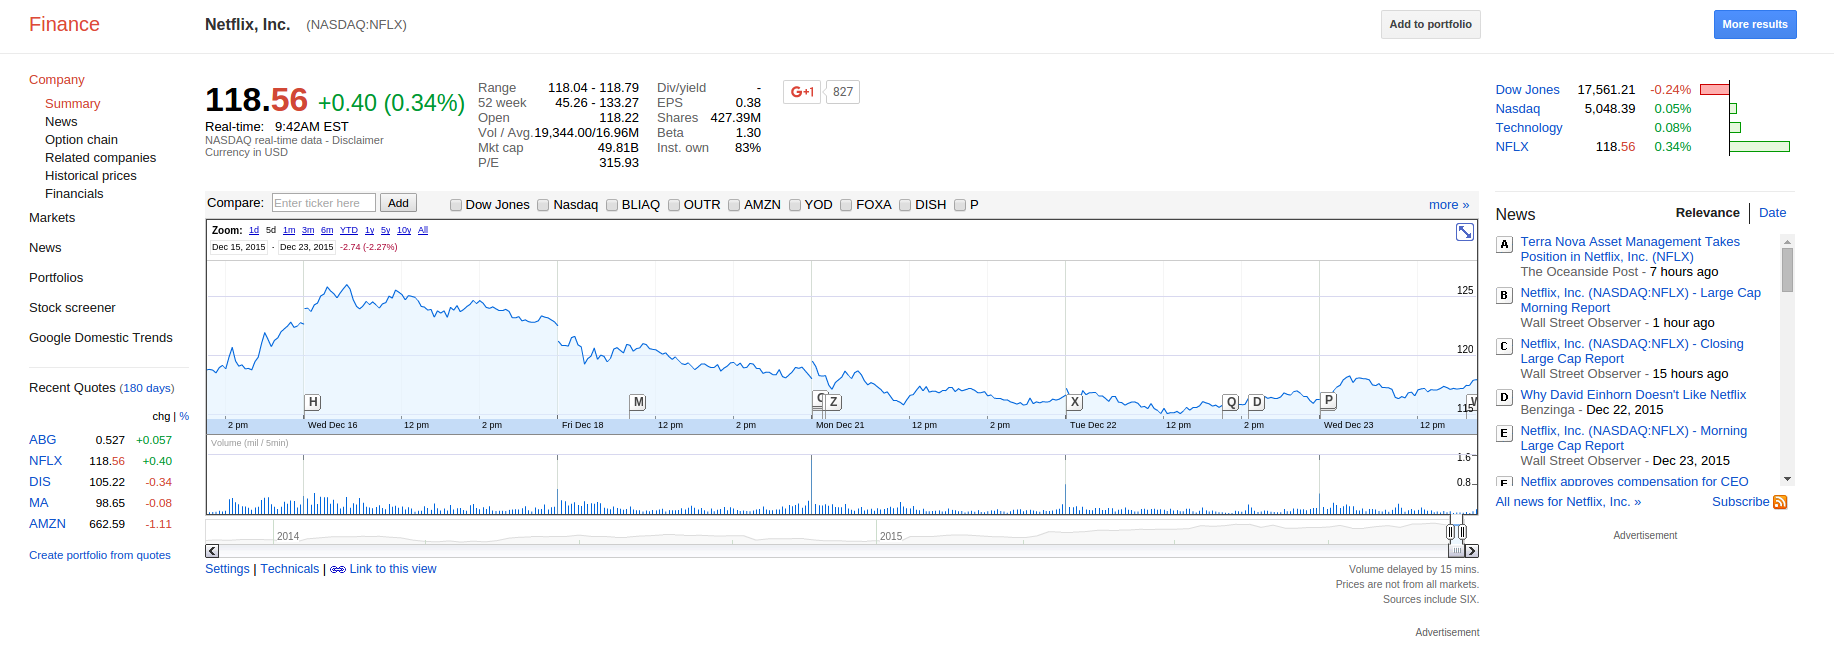
\includegraphics[width=1.2\textwidth]{img/netflix.png}
\label{fig:netflix}
\end{center}
\end{adjustwidth}

Si nos fijamos en la silueta de la gráfica mostrada podemos ver que el precio de las acciones subió hace cuatro días pero ha ido bajando desde entonces. Esta silueta nos permite ver la situación de la empresa cuyo precio en el mercado ha bajado recientemente.

No obstante, podemos ver que la figura no es suave en absoluto sino que oscila continuamente. Estas oscilaciones se deben a la compra y venta de acciones que se producen constantemente en el mercado.

Cuando el precio de la acción baja, y los corredores de bolsa consideran que ha bajado lo suficiente, comienzan a comprarse acciones lo que hace que la demanda suba y con ella el precio.

Llegados a cierto punto, los accionistas consideran que la acción ha subido lo suficiente de precio y deciden venderla. En este momento la demanda se reduce drásticamente aumentando la oferta con lo que el precio de la acción baja.

Si decidimos invertir en bolsa, debemos estar atentos y tener una óptima conexión de forma que logremos comprar en el momento óptimo (precio mínimo de la acción) y venderla cuando esta alcanza su precio máximo.

\section{Administración}

\subsection{Nóminas, Seguridad Social e IRPF}

Las nóminas financian al Estado a través de dos ``agencias'': la Agencia Tributaria (Hacienda) y la Tesorería General de la Seguridad Social (TGSS).

Un trabajador tiene un salario bruto mensual $S_B$, del que se deduce una cantidad $I_S$ para la TGSS y otra $I_I$ para el IRPF\footnote{Impuesto sobre la Renta de las Personas Físicas, gestionado por la Agencia Tributaria.}. Además, la empresa paga a la TGSS otra cantidad $I_{SE}$ según el salario bruto del trabajador.

\subsubsection{Seguridad Social}

\begin{table}[hbtp]
\centering
\footnotesize
\begin{tabular}{l|r|r|r}
\textbf{Contingencia} & \textbf{Empresa} & \textbf{Trabajador} & \textbf{Total} \\ \toprule
Común - Tipo general & 23.60 & 4.70 & 28.30 \\
Común - Horas extra fuerza mayor & 12.00 & 2.00 & 14.00 \\
Común - Resto horas extra & 23.60 & 4.70 & 28.30 \\ \midrule
Desempleo - Tipo general & 5.50 & 1.55 & 7.05 \\
Desempleo - Contrato temporal a tiempo completo & 6.70 & 1.60 & 8.30 \\
Desempleo - Contrato temporal a tiempo parcial & 6.70 & 1.60 & 8.30 \\ \midrule
Fondo de Garantía Salarial (FOGASA) & 0.20 & 0 & 0.20 \\ \midrule
Formación Profesional & 0.60 & 0.10 & 0.70 \\ \midrule
Accidentes de trabajo y enfermedades profesionales & ($\ast$) & 0 & ($\ast$) \\ \midrule
\end{tabular}
\caption{\study{Tipos} (en porcentaje) \study{de cotización}, separando qué porcentaje recae en la empresa y qué porcentaje en el trabajador. La parte de ($\ast$) corresponde a la tarifa de primas que varía según trabajador.}
\label{tab:TiposSegSocial}
\end{table}

Las cotizaciones a la Seguridad Social vienen reguladas por la orden ministerial correspondiente de cada año. En 2015, aparecen en la \href{http://www.boe.es/diario_boe/txt.php?id=BOE-A-2015-847}{Orden ESS/86/2015}. Los tipos de cotización se pueden ver en la \fref{tab:TiposSegSocial}.

Las contingencias para accidentes de trabajo y enfermedades profesionales dependen de la empresa y el puesto del trabajador, según la \href{http://www.seg-social.es/Internet_1/Trabajadores/CotizacionRecaudaci10777/TarifadePrimasdeATy48410/index.htm}{tarifa de primas vigente}: se aplica el porcentaje de cotización correspondiente según la actividad económica de la empresa (Cuadro I que aparece en el PDF de la tarifa de primas) salvo que el trabajador entre en alguna de las ocupaciones del Cuadro II de la tarifa de primas, en cuyo caso será el tipo del Cuadro II el que se aplique.

\paragraph{Cálculo de la aportación a la SS} Para el cálculo de la aportación, lo primero que se hace es calcular la \study{base de cotización}. Ésta está conformada por el \substudy{salario bruto}, sin contar indemnizaciones o compensaciones de gastos\footnotemark, e \substudy{incluyendo las pagas extras prorrateadas} (esto es, si tenemos dos pagas extras de $x$ euros cada una, al salario bruto para un mes de $d$ días tendremos que añadirle la parte proporcional de las pagas extras, $\frac{d}{365} \cdot 2x $).
De este resultado, debemos \substudy{contar por separado las horas extras} y aplicarles el tipo correspondiente de contingencias comunes de la \fref{tab:TiposSegSocial} según sean \substudy{horas de fuerza mayor} (las empleadas para prevenir o reparar siniestros o daños extraordinarios, como terremotos, incendios o similares) o no.
El resto de contingencias (desempleo, FOGASA, etc) se aplican al total de salario bruto.

Un detalle a la hora de calcular la base de cotización es que hay \href{http://www.seg-social.es/Internet_1/Trabajadores/CotizacionRecaudaci10777/Basesytiposdecotiza36537/index.htm}{\study{mínimos y máximos de cotización}} según puesto y contingencia: si la base no está en ese intervalo, ya sea porque estamos por debajo o por encima, usaremos el mínimo o el máximo respectivamente a la hora de calcular la cuota.

\footnotetext{Ver \href{http://www.seg-social.es/Internet_1/PortalEducativo/Profesores/Unidad6/Cotizacionregimengeneral/Basedecotizacion/Composiciondelabasedecotizacion/index.htm}{la web de la SS} para algunos ejemplos, el \href{http://www.seg-social.es/Internet_1/Normativa/095235?ssSourceNodeId=292}{artículo 23 del Reglamento general sobre cotización y liquidación de 1995 (que supongo sigue vigente)} para el reglamento concreto y \href{http://www.seg-social.es/prdi00/groups/public/documents/binario/178628.pdf}{este boletín de la SS} para una tabla con las deducciones concretas.}

\subsubsection{IRPF}

Cada año (más concretamente, cada ejercicio fiscal), las personas físicas deben hacer la declaración de la renta\footnote{Sólo es obligatorio habiendo recibido más de 22.000 euros brutos de un pagador o más de 11.200 euros de dos pagadores, con el segundo y siguientes pagando más de 1.500 euros.} y pagar un impuesto en base a los ingresos (renta) que haya tenido.

Para evitar el susto en la declaración, las actividades económicas están sujeta a retención. Así, cuando un empleador paga a un empleado, una parte se va a Hacienda retenida en concepto de IRPF\footnotemark.
Es en la declaración de la renta donde se echan cuentas y se ve si hemos pagado de más o de menos a Hacienda.

\footnotetext{\href{http://www.agenciatributaria.es/static_files/AEAT/Contenidos_Comunes/La_Agencia_Tributaria/Informacion_institucional/Campanias/IRPF_permanente/Informacion_general/Cuestiones_destacadas/reten_ingresos_cuenta_IRPF.pdf}{Aquí los tipos de retención} según la actividad económica, y aquí el \href{http://www.agenciatributaria.es/AEAT.internet/Inicio/La_Agencia_Tributaria/Campanas/Retenciones/Ejercicio_2015__hasta_11_de_julio__o_en_su_caso__31_de_julio_/Informacion_tecnica/Informacion_tecnica.shtml}{algoritmo concreto} (horrible) que usan. En la \href{http://www.agenciatributaria.es/AEAT.internet/Retenciones.shtml}{Agencia Tributaria} está el resto de información necesaria, como un simulador de retenciones.}

La cantidad a pagar a Hacienda depende de un montón de aspectos\footnote{Cosas que deberían aparecer todas en la \href{https://www.boe.es/buscar/act.php?id=BOE-A-2006-20764&tn=1&vd=&p=20151030}{Ley 35/2006} sobre el IRPF y sus sucesivas modificaciones (\href{http://www.boe.es/diario_boe/txt.php?id=BOE-A-2015-7765}{la última, de 2015}.)}.
La \study{base imponible} se calcula como la \substudy{suma de nuestros ingresos declarados (}\study{sin}\substudy{ incluir las cotizaciones a la }\study{Seguridad Social}), \substudy{quitando} los que estén exentos (por ejemplo, \substudy{ayudas}, subvenciones).

Además, a partir de la reforma fiscal que entra en vigor en 2015, se añade una partida más en concepto de ``gastos generales''\footnote{Ver artículo 19.2.f) de la \href{https://www.boe.es/buscar/act.php?id=BOE-A-2006-20764&b=29&tn=1&p=20141128}{Ley del IRPF}.}, de tal forma que además del mínimo, hay que \substudy{restar 2.000 euros} más de la base imponible (así que pagamos menos impuestos).


Por último, existe un \substudy{mínimo personal y familiar}, que como mínimo es de \substudy{5.550} euros y depende de los hijos que tenga uno a su cargo, discapacidades y demás\footnote{Ver artículos 56 a 60 de la \href{https://www.boe.es/buscar/act.php?id=BOE-A-2006-20764&b=29&tn=1&p=20141128}{Ley del IRPF}.}.
Esta cantidad está exenta de tributar, pero computa dentro de los 12.450\texteuro.


En la tabla \ref{tab:Tramos2015IRPF} vemos los tramos del IRPF contemplados por la ley. En la tabla \ref{tab:Tramos2015IRPF_FMM} vemos los tramos del IRPF una vez incluidos el mínimo personal y familiar.
Incluimos esta segunda tabla para ejemplificar que el mínimo personal y familiar computa de una manera distinta a los "gastos generales". Ambos no tributan impuestos, pero unos computan como parte de ingresos en la base imponible (mínimo) mientras que los "gastos generales" no forman parte de la base imponible.

La respuesta a ¿Por qué no se construye siempre la tabla simplificada? Porque ese mínimo de 5500 depende de varios factores y los 2000 fueron una pequeña modificación.


\begin{table}[hbtp]
\centering
\footnotesize
\begin{tabular}{r|r|r|r|r}
\textbf{Desde} & \textbf{Hasta} & \textbf{Longitud tramo} & \textbf{Cuota íntegra} & \textbf{Tipo aplicable} \\ \toprule
0 & 12,450 & 12,450 & 0.00 & 19.5 \\
12,450 & 20,200 & 7,750 & 2,427.75 & 24.5 \\
20,200 & 34,000 & 13,800 & 4,326.50 & 30.5 \\
34,000 & 60,000 & 26,000 & 8,535.50 & 38.0 \\
60,000 & $\infty$ & $\infty$ & 18,415.50 & 46.0 \\
\end{tabular}
\caption{Tramos del IRPF para el ejercicio fiscal 2015 según la ley.}
\label{tab:Tramos2015IRPF}
\end{table}

\begin{table}[hbtp]
\centering
\footnotesize
\begin{tabular}{r|r|r|r|r}
\textbf{Desde} & \textbf{Hasta} & \textbf{Longitud tramo} & \textbf{Cuota íntegra} & \textbf{Tipo aplicable} \\ \toprule
0 & 5.500 & 5.500 & 0,00 & 0,0 \\
5500 & 12.450 & 6.950 & 0,00 & 19,5 \\
12.450 & 20.200 & 7.750 & 1.355,20 & 24,5 \\
20.200 & 34.000 & 13.800 & 3.253,90 & 30,5 \\
34.000 & 60.000 & 26.000 & 7462,90 & 38,0 \\
60.000 & $\infty$ & $\infty$ & 17.343,43 & 46,0 \\
\end{tabular}
\caption{Tramos del IRPF para el ejercicio fiscal 2015 a utilizar,  simplificando (sin perder precisión) computando el mínimo personal y familiar de manera sencilla.}
\label{tab:Tramos2015IRPF_FMM}
\end{table}


El \substudy{porcentaje de impuesto efectivo} no es el del tramo en el que esté tu base liquidable, sino la \substudy{media ponderada} según los tramos.
Lo de la \textbf{cuota íntegra} es simplemente una ayuda para calcularlo: la cuota íntegra de un tramo es el resultado de aplicar a todos los tramos anteriores su gravamen correspondiente, de tal forma que sólo tengas que calcular el porcentaje para lo que lleves del último tramo y sumarle la cuota íntegra.

Por último, en enero de 2016 entra en vigor una nueva ley del IRPF en la que se cambian los tramos, los porcentajes, las deducciones... pero el esquema de cálculo se sigue manteniendo.

\subsubsection{Cuánto paga la empresa}
Hay que destacar que no sólo es el trabajador el que paga el impuesto de la Seguridad Social y el IRPF. Por cada pago que realiza el trabajador (que, como se ha explicado con anterioridad, es pagado directamente por la empresa sustrayendo el importe correspondiente del salario del trabajador), la empresa también tiene que pagar una cantidad, tanto de impuesto de Seguridad Social como IRPF aún mayor que lo que paga el trabajador.

\subsubsection{Ejemplo de una nómina}
La \fref{tab:EjemploNomina} muestra un ejemplo de nómina de un trabajador, viendo cuánto cobra en neto y cuánto tiene que pagar la empresa. El salario bruto es 18.000\texteuro , la seguridad social por parte del trabajador 6,35\% y por parte de la empresa 31\%.


\paragraph{Seguridad Social}
Sabemos que el porcentaje de seguridad social aplicado es del 6,35\%, con lo que la cotización a la seguridad social por parte del trabajador será
\[6,35\% · 18.000 = 1.143 \]

\paragraph{IRPF} El cálculo del IRPF es algo más complejo.

El salario bruto son 18.000 \texteuro . Para calcular el tipo de IRPF calculamos la base imponible:
\[
B_l = 18.000 - 2.000 - 1.143 = 14857,00
\]

\begin{table}[hbtp]
\centering
\begin{tabular}{l||r|r|r}
De 0 a 5.500 & 5.500 & 0 & 0\\
De 5.500 a 12.450 & 6.950 & 19,5\% & 1.355,25\\
De 12.450 a 14.857 & 2.407 & 24,5\% & 589.72\\ \bottomrule
Total & & & 1.945,00
\end{tabular}
\caption{Cálculo del IRPF}
\end{table}

Y ahora podemos calcular el tipo aplicado (el porcentaje equivalente):\footnote{El simulador de la agencia tributaria da un resultado similar, pero no exactamente igual}

\[
	\frac{6950*19.5 + 2407*24.5}{18000} = \frac{1945}{18000} = 10.80
\]

En la tabla \ref{tab:EjemploNomina} encontramos de manera resumida el desglose de la nómina, incluyendo la cotización por parte de la empresa.

\begin{table}[hbtp]
\centering
\begin{tabular}{l||r|r||r|r}
\multicolumn{1}{c}{} & \multicolumn{2}{c}{\textit{Trabajador}} & \multicolumn{2}{c}{\textit{Empresa}} \\ \toprule
\textbf{Concepto} & \textbf{Mensual} & \textbf{Anual} & \textbf{Mensual} & \textbf{Anual} \\ \toprule
Salario Bruto & 1.285,71 \texteuro & 18.000,00 \texteuro & 1.285,71 \texteuro & 18.000,00 \texteuro \\
Seguridad Social & 95,25 \texteuro & 1143,00 \texteuro & 465,00 \texteuro & 5.580,00 \texteuro \\
IRPF & 138,93 \texteuro & 1.945,00  \texteuro & 0,00 \texteuro & 0,00 \texteuro \\ \bottomrule
Neto & 1.051,9 \texteuro & 14.912,00 \texteuro & 1750,71 \texteuro & 23.580,00 \texteuro
\end{tabular}
\caption{Un ejemplo de nómina, con tipo de IRPF 10,8\% y Seguridad Social de 6,35\% a cargo del trabajador y 31\% a cargo de la empresa.}
\label{tab:EjemploNomina}
\end{table}

Es decir, si el trabajador recibe un neto de 1.051,9 \texteuro \ al mes, la empresa debe pagar un total de 1750,71 \texteuro \ al mes y el estado recibe casi 700 \texteuro  cada mes.



\paragraph{Reducción por rendimiento de trabajo}

Aunque no se ha visto en clase, consideramos importante su inclusión aquí. Vamos a ver una de las muchas deducciones que existe en el IRPF. Hemos considerado esta importante porque sólo depende de la renta y es general, no como las reducciones por número de hijos, edad o residencia geográfica.

\begin{itemize}
\item Contribuyentes con ingresos iguales o inferiores a 11.250 euros tiene exentos 3.700 euros anuales.
\item Contribuyentes con ingresos comprendidos entre 11.250 y 14.450 euros tiene exentos $(3.700  - 1,15625 · (\text{ingresos} - 11.250))$.
\end{itemize}

Esta deducción supone que rentas inferiores a 11.959\texteuro no pagan IRPF, ya que $2000+5500+3700+6.35\% · (11.959) = 11.959$ (suponiendo correcto el porcentaje de Seguridad Social retenido).

\subsection{Facturación, ventas y cobros. IVA}

Una factura es, formalmente, un documento con toda la información de una compraventa. Lo emiten los que pueden vender, esto es, autónomos o empresas. La factura siempre ha de incluir el IVA correspondiente a lo que se venda, según los \href{http://www.agenciatributaria.es/static_files/AEAT/Contenidos_Comunes/La_Agencia_Tributaria/Segmentos_Usuarios/Empresas_y_profesionales/Novedades_IVA_2014/Nuevos_tipos_IVA.pdf}{tipos que establezca la AEAT}
(principalmente hay tres: \substudy{general del 21 \%, reducido del 10 \% y superreducido del 4 \%}).

El IVA, \concept{Impuesto\IS sobre el Valor Añadido}\index{IVA}, es un impuesto que recae sobre el consumidor, y que gestionan los autónomos y empresas para el Estado. Cuando le vendemos un producto a un consumidor, le cobramos el precio que queramos y además le pedimos un porcentaje de ese precio en concepto de IVA.
Esa cantidad va directa al Estado en la \study{declaración trimestral del IVA}.

Cuando la venta se la hacemos a otra empresa o autónomo (esto es, no a un consumidor), seguiremos cobrándole el IVA igualmente y dándoselo al Estado. El otro deberá luego deducirse esa cantidad de IVA que nos ha pagado en su declaración del IVA, para que el Estado se la devuelva\footnote{En la práctica no se devuelve, simplemente miran cuánto IVA ha pagado la empresa y cuánto ha cobrado y le ingresa a Hacienda la diferencia - normalmente, las empresas cobran más IVA que el que pagan.}.

Esto desencadena en algunos problemas como nos muestra el siguiente ejemplo, utilizado por el profesor en clase en diversas ocasiones:
\begin{example}
Si desarrollas un Software para el Corte Inglés y quieres ganar $X$ cantidad de dinero con él, se lo tendrás que vender al cliente por el precio $X+$IVA$\times X$.

No obstante, puesto que el Corte Inglés va a deducirse el IVA, es decir, le van a reembolsar lo que te pague de IVA, le interesa recibir esa ``devolución'' antes de haber pagado.

Por tanto, el IVA te exigirá la emisión de la factura lo antes posible aunque la empresa no va a pagarte hasta, por lo menos, un año más tarde.

Puesto que la factura ya ha sido emitida, el Corte Inglés ya puede deducirse el supuesto IVA (que aún no ha pagado) con lo que el Estado le paga. El problema es que esto también implica que tu, como cliente, debes pagar tu IVA (el que le ibas a cobrar al Corte Inglés), aunque este no haya pagado.

Es decir, le vendes un Software a una gran empresa y no sólo tardarás en cobrar sino que, además, deberás pagar el IVA de un beneficio que aún no has percibido.
\end{example}

A raíz de situaciones como la del ejemplo, el estado trató de cambiar las cosas, permitiendo al autónomo del ejemplo no pagar el IVA hasta que recibiera el cobro. No obstante, esto implicaba que el Corte Inglés tampoco recibiría ese IVA hasta pagar.

Finalmente muy pocos autónomos o pequeñas empresas se acogieron a esta posibilidad puesto que esto les implicaba que grandes empresas como el Corte Inglés en el ejemplo, dejasen de contratar sus servicios.

\obs La declaración del IVA se realiza de manera trimestral.

A la pregunta sobre si se ha de facturar o no, la respuesta es sencilla. Si se trata de ingresos esporádicos, no muy grandes y a particulares, teniendo en cuenta el engorro y los costes de hacerse autónomo, lo mejor es buscar formas alternativas de declarar esos impuestos. Si no, probablemente necesites hacerte autónomo. En cualquier caso, siempre hay que declarar los ingresos y pagar los impuestos correspondientes.

\subsubsection{Herencias}

Aunque no se ha dedicado ninguna clase a la explicación detallada de los impuestos que afectan a las herencias, si que se ha comentado en más de una ocasión. \footnote{Incluímos este tema dentro de este capítulo por estar intimamente ligado al tema de los impuestos.}


En el momento de recibir una herencia, hay dos aspectos a tener en cuenta \textbf{muy importantes} y que la gente, por lo general, desconocer.

\begin{enumerate}
\item Al hablar de la \study{herencia positiva}, la que supone un incremento de riqueza del beneficiario, esta herencia viene acompañada de impuestos.

Esto no sería tan malo, a priori, pues el impuesto es un porcentaje de lo que recibes, por lo que simplemente reduce la cantidad a recibir.

El problema grave es que los \study{impuestos} deben \study{pagarse antes de recibir} la herencia.
Por tanto, atendiendo a una simulación realizada a través de una aplicación online y que recoge la figura \fref{fig:impuestoHerencia}, si nos disponemos a recibir una herencia de 500.000 \texteuro \ (supongamos que el difunto ganó la lotería poco antes del fallecimiento), el beneficiario de la herencia se ve obligado a pagar más de 100.000 \texteuro antes de poder tener acceso a esa herencia.

Por tanto, en lugar de dinero, lo que se recibe es una deuda por valor del impuesto correspondiente que debe ser pagada. No obstante, siempre puede renunciarse a la herencia con lo que deja de ser necesario el pago de esta deuda.

\begin{figure}[hbtp]
\centering
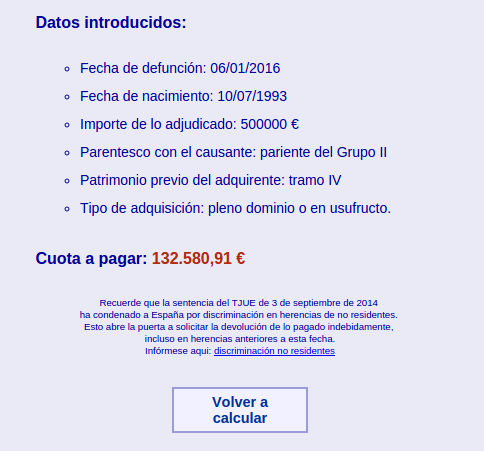
\includegraphics[width=0.7\textwidth]{img/simulacion_sucesiones.png}
\caption{Impuestos vinculados a una herencia}
\label{fig:impuestoHerencia}
\end{figure}

Es importante destacar también que \substudy{los impuestos de cada comunidad autónoma de España son distintos}, por eso hay quienes dicen que mucha gente \textit{viene a morir a Madrid}, porque en la comunidad autónoma de Madrid están los menores impuestos de sucesión.


\item Por otro lado también se recibe una \study{herencia negativa}.
Las \study{deudas} que tuviera el difunto, en principio, parecen perderse pero el banco tiene el derecho a indagar, encontrar al heredero y hacerle pagar la deuda.
Además de las deudas, también se heredan los \study{avales}.
Si el fallecido avaló un préstamo, el heredero asume la responsabilidad del pago de ses préstamo, ya se se convierte en avalador.

\end{enumerate}

¿Y si la herencia negativa es mayor que la positiva? Entonces puedes renunciar en su totalidad a la herencia y esta pasará al Estado o a la Comunidad Autónoma. \substudy{Las herencias se aceptan en su totalidad o se rechazan en su totalidad}. O todo o nada de nada.
\footnote{En clase se comentó la posibilidad de que el banco podía ir tras los herederos para intentar que ellos paguen la deuda del fallecido. El banco, por poder, puede ir. Nadie le impide presionar, demandar etc Pero el heredero, si ha renunciado, puede pasar del banco legítimamente.}

No obstante hay una posibilidad "intermedia" que se denomina \concept{beneficio de inventario}, en la que se otorga la posibilidad de no tener que responder con patrimonio propio a las deudas de una herencia, sino únicamente con la propia herencia.
Eso sí, es un trámite muy burocrático, muy chungo con muchos pasos que dar y como te equivoques en algo, se considera que has aceptado la herencia en su totalidad.

Además, en las herencias hay 2 posibles receptores, los herederos y los legatarios.
El \substudy{heredero sucede al fallecido} en su conjunto patrimonial, activo y pasivo, \substudy{tanto en los derechos como en las obligaciones} que no se extingan por su muerte, mientras que el \substudy{legatario sólo} lo hace en \substudy{bienes o derechos} determinados por el fallecido.
Tras esto, pensarás ¿Por qué no ser todos legatarios siempre?
Porque es \substudy{necesario que exista un heredero} que suceda al fallecido. El heredero (o herederos) es el encargado de gestionar la herencia y darle a los legatarios su legado.
En caso de repartir una herencia entre únicamente legatarios, éstos se convertirán en herederos, porque esta figura es necesaria.


\subsection{Certificados digitales}

Bueno, esto no merece mucha explicación. Las administraciones públicas emiten certificados digitales (hay que pedirlo y luego personarse en la administración que corresponda con documentos que acrediten tu identidad como persona física o jurídica) para operar con ellas a través de Internet.

A estas alturas de la carrera, todo informático que se precie debe entender perfectamente qué son los certificados digitales y cómo funciona.

\subsection{Contratos}

\begin{table}[hbtp]
\centering
\begin{tabular}{l|l|l}
\textbf{Despido} & \textbf{Días por año trabajado} & \textbf{Mensualidades máximas} \\ \toprule
Procedente & 20 & 12 \\
Disciplinario & 0 & 0 \\
Improcedente & 33 & 24 \\
Fin contrato temporal & De 8 a 12 & - \\
\end{tabular}
\caption{Tabla con las indemnizaciones por despido.}
\label{tab:Despido}
\end{table}

Los contratos pueden ser de diferentes tipos, principalmente se dividen en fijos y temporales (estos pueden ser por obra y servicio, por tiempo...). También hay contratos de formación y de prácticas.

Una vez que se contrata a un empleado, se le puede despedir\footnote{Un despido es una anulación del contrario por parte del contratante} previo pago de la correspondiente indemnización, que dependerá, entre otros, del tiempo que se trabaje (días por año trabajado, añadiendo la parte proporcional a los períodos inferiores a un año) y el tipo de despido, según la \fref{tab:Despido}.
Describimos a continuación los \study{tipos de despido}\footnote{Ver la sección cuarta del \href{https://www.boe.es/buscar/act.php?id=BOE-A-1995-7730&tn=1&p=20151024}{Estatuto de los trabajadores}}:

\begin{itemize}
\item \concept{Despido\IS procedente}. Se extingue el contrato por ineptitud del trabajador conocida o sobrevenida después de la contratación y del período de prueba, por faltas de asistencia o por faltas de adaptación a cambios razonables en el puesto de trabajo. También se podrá efectuar un despido por causas económicas de la empresa.
\item \concept{Despido\IS disciplinario}. Se extingue el contrato por incumplimiento grave y culpable del trabajador, como faltas repetidas e injustificadas, indisciplina, ofensas verbales o física, acoso y similares.
\item \concept{Despido\IS improcedente}. Cuando se modifiquen las condiciones de trabajo del empleado sustancialmente sin respetar el artículo 41 del Estatuto de los trabajadores, falta de pago u otro incumplimiento grave del empresario (el trabajador tendrá que solicitar en el juzgado de lo social la extinción). También habrá despido improcedente si un juez lo determina así.
\end{itemize}

Además, cuando se acaba un contrato temporal, e trabajador tendrá derecho a doce días de salario por cada año de servicio\footnote{Ver \href{http://www.empleo.gob.es/es/Guia/texto/guia_7/contenidos/guia_7_16_4.htm}{la web del Ministerio de Empleo} para los detalles exactos.}.

\section{Análisis de estados financieros}

\begin{defn}[Contabilidad]
La contabilidad se puede definir, en palabras del profesor, como una técnica que permite construir e interpretar estados financieros.
\end{defn}

El análisis de estados financieros de una empresa implica, como su nombre indica, \study{analizar y diseccionar el estado del dinero en una empresa}. Se podrían distinguir dos ámbitos de contabilidad:

\begin{itemize}
\item \textbf{Contabilidad \study{financiera}}. Es un \substudy{registro} sistemático \substudy{de} las \substudy{operaciones} que la empresa realiza con el \substudy{exterior}.

Forman parte de la contabilidad financiera, por ejemplo, los préstamos pedidos, la compra de material, los pagos a Hacienda, las ventas, la compra de edificios, ...

Esta contabilidad se lleva con el objetivo de llevar un control y \textbf{es \study{obligatoria}}. Sirve para \substudy{conocer el patrimonio de la compañía y los resultados de la empresa}.

Si bien algunos conceptos pueden ser ambiguos a la hora de estudiarlos, \substudy{existen} una serie de \textbf{\substudy{estándares}} que nos dicen cómo proceder.

\item \textbf{Contabilidad de costes} Tiene como objetivo conocer los costes, los \substudy{márgenes de beneficios} y las contribuciones de los socios.

En general \substudy{depende} enormemente de la \substudy{estructura interna} de la empresa por lo que no está estandarizada y no existen programas informáticos que ayuden en esta tarea.
\end{itemize}

En esta sección nos centraremos en el estudio de la \textbf{contabilidad financiera}.

\subsection{Contabilidad: Balance, PyG y caja}
\label{sec:Contabilidad}

Las \substudy{empresas españolas} están \substudy{obligadas a presentar las cuentas anuales} en el registro mercantil según el \href{https://www.boe.es/buscar/doc.php?id=BOE-A-2007-13023}{\substudy{Plan General Contable} de 2007}, corregido en la \href{https://www.boe.es/boe/dias/2009/02/10/pdfs/BOE-A-2009-2276.pdf}{Orden JUS/206/2009 del 28 de enero}.

\subsubsection{Técnica de contabilidad: Asientos}

\begin{table}[hbtp]
\centering
\begin{tabular}{r|p{5cm}||p{5cm}|l}
\textbf{Debe} & \textbf{Concepto} & \textbf{Concepto} & \textbf{Haber} \\ \toprule
1.096,25 & (640) Sueldos y salarios & (476) Organismos de la Seg. Social. acreedores & 480,81 \\
372,63 & (642) S.S. a cargo de la empresa & (4751) Hac. Pública acreedor por retenciones practicadas & 94,27 \\
 & & (465) Remuneraciones pendientes de pago & 893,8 \\ \midrule
 893,8 & (465) Remuneraciones pendientes de pago & (572) Bancos c/c & 893,8 \\ \midrule \midrule
10.000 	& (600) Compra de mercaderías & (400) Proveedores &	12.100 \\
2.100 	& (472) H.P. IVA Soportado & &  \\ \midrule
12.100 	& (400) Proveedores & (572) Bancos e instituciones bancarias &	12.100 \\ \midrule \midrule
12.100 	& (430) Clientes & 	 (700) Venta de mercaderías & 10.000 \\
 & & (477) H.P. IVA Repercutido & 2.100 \\ \midrule
12.100 & (572) Bancos c/c & (430) Clientes & 12.100 \\
 \bottomrule
\end{tabular}
\caption{Ejemplo de asientos contables. El primer asiento corresponde al pago de un salario: sale dinero de la cuenta de sueldos y salarios (lo que en el PyG aparecerá como sueldos y salarios) y de la cuenta de la seguridad social a cargo de la empresa. Ese dinero se va a la Seguridad Social (la parte de cotización de la SS de la empresa y la parte del trabajador), a la hacienda pública (el IRPF retenido) y a remuneraciones pendientes de pago. En el siguiente asiento, sacamos las remuneraciones pendientes de pago y las pagamos a través del banco. En los dos siguientes asientos, hacemos una compra de material. El tercer grupo de asientos es un ejemplo de cómo contabilizaríamos una venta pagada por entidad bancaria (si fuese al contado, en lugar de Bancos tendríamos Caja). En los dos últimos grupos de asientos, el primer asiento corresponde a cuando se hace la venta, y el segundo a cuando se hace el cobro efectivo.}
\label{tab:Asientos}
\end{table}

La técnica contable lleva la lista de asientos. Un \concept{Asiento} es simplemente el registro de una operación. Cada cuenta tiene dos partes: el lado del debe llamado \textbf{\substudy{partida}} (\substudy{izquierdo}) y el lado del haber llamado \textbf{\substudy{contrapartida}} (\substudy{derecho}).
Esto quiere decir que una cuenta puede incrementar o aminorar su saldo según las operaciones que se realicen.
Estos aumentos y disminuciones tienen un nombre: \concept{Cargo} y \concept{Abono}.\footnote{
 \href{http://www.plangeneralcontable.com/?tit=guia-de-contabilidad-para-torpes&name=GeTia&contentId=man_ctorpes&manPage=8}{En esta página} se puede encontrar una descripción más detallada de estos conceptos.}


Se llama \substudy{cargar} en una cuenta, a registrar una operación en el \substudy{debe} de dicha cuenta.

Se llama \substudy{abonar} en una cuenta, a registrar una operación en el \substudy{haber} de dicha cuenta.

De manera obvia si alguien gana es porque otro lo pierde. Nuestro objetivo al estudiar la contabilidad es saber \study{quién gana}, \study{quién pierde} y qué consecuencias tiene esto. Este es el principio de \textbf{\study{partida doble}}.

Las cuentas de donde sale y entra el dinero están definidas según el PGC\footnote{\href{https://www.boe.es/boe/dias/2007/11/20/pdfs/C00001-00152.pdf}{Plan General de Contabilidad}.}. La \fref{tab:Asientos} tiene un ejemplo con varias operaciones y su descripción.

%Adicionalmente, sería relevante revisar qué pasa con las cuentas de bancos y de otros activos en general. La cuestión es que cuando una cuenta de activo aparece en el ``debe'', esta cuenta aumenta (por ejemplo, cuando ponemos la cuenta de Bancos en el debe, significa que nuestro activo por dinero en bancos aumenta), y disminuye cuando aparece en el haber. Análogamente, cuando una cuenta de pasivo aparece en el haber, su cantidad aumenta; y si aparece en el debe, su cantidad disminuye.

Al final, todos esos asientos se suman (el haber es positivo, el debe es negativo) y sale la \concept{Mayor}. El debe y el haber deberían sumar lo mismo al hacer el mayor de todas las cuentas ya que, de no ser así, significaría que estamos creando dinero de la nada.

En el apéndice \ref{sec:contabilidad} podemos encontrar un esquema que resume los conceptos que acabamos de ver sobre la \textbf{contabilidad}, acompañado de un ejemplo.

\subsubsection{Determinación de rendimientos para el IRPF de autónomos}

Cuando uno lleva a cabo una actividad económica (esto es, es autónomo), tenemos dos formas\footnotemark de estimar nuestros rendimientos netos y por lo tanto dos métodos de decirle a Hacienda cuál es nuestra base imponible sobre la que se aplican los impuestos.

\footnotetext{Esto aparece en el \href{https://www.boe.es/buscar/act.php?id=BOE-A-2006-20764}{artículo 16.2 de la ley del IRPF}, y se desarrollan los regímenes en el \href{https://www.boe.es/buscar/act.php?id=BOE-A-2007-6820}{artículo 27 del Real Decreto 439/2007}.}

Existen dos regímenes de estimación: la \study{directa} (con \substudy{dos modalidades}) y la \study{objetiva}.

El \concept{Régimen\IS de estimación directa simple} es el \study{método por defecto}, que sólo deja de aplicarse \substudy{si renunciamos a él o} si la \substudy{cifra de negocio (las ventas que tenemos quitadas deducciones e IVA}\footnote{Definido en el \href{http://www.boe.es/buscar/doc.php?id=BOE-A-1989-30361}{artículo 191 de un RDL derogado}, aunque parece que la cifra no ha cambiado.}) \substudy{supera los 600.000 euros anuales}.
La \substudy{base imponible} se calcula como los \substudy{ingresos menos los gastos y deducciones}, \substudy{incluyendo} además una \substudy{deducción del 5\% del rendimiento neto} del ejercicio anterior para provisiones y gastos de difícil justificación.
Hay además \href{http://portal.circe.es/es-ES/emprendedor/EmpresarioIndividual/TributacionAutonomos/Paginas/AutonomoEstimacionDirectaSimplificada.aspx}{otros pequeños detalles}.

El \concept{Régimen\IS de estimación directa normal} se utiliza cuando la cifra de negocio \substudy{supera los 600.000 euros anuales}.
En estos casos la \substudy{base imponible} se calcula igual pero \substudy{añadiendo el autoconsumo}\footnote{Ver \href{http://www.pymesyautonomos.com/fiscalidad-y-contabilidad/el-autoconsumo-de-bienes-y-servicios-tratamiento-fiscal-y-contable}{este sitio} para una explicación, básicamente es cuando el autónomo consume sus propios servicios.} a los ingresos. \href{http://portal.circe.es/es-ES/emprendedor/EmpresarioIndividual/TributacionAutonomos/Paginas/autonomoestimacionDirectaNormal.aspx}{Aquí hay más detalles}.

Estos dos casos requieren que el autónomo lleve control de su contabilidad. No obstante, en ocasiones, esto escapa de la formación/preparación del autónomo en cuestión.

Por ejemplo, en el caso de un taxista, es frecuente que no lleve un control detallado de la contabilidad y por tanto sea incapaz de acogeres a uno de los dos métodos de estimación del IRPF que acabamos de ver.

Para casos como este, Hacienda tolera que algunas personas no lleven la contabilidad de su negocio (ya sea porque no pueden o porque no quieren hacerlo). En estos casos es Hacienda la que calcula, en lugar del propio autónomo, cuáles son sus ganancias.

Como hacienda no tiene datos sobre la situación real del negocio, lo que hace es una estimación basándose en estadísticas y en variables objetivas del negocio. Esto es lo que se conoce como \textbf{régimen} de estimación objetiva.


El \concept{Régimen\IS de estimación objetiva}\footnote{Regulado en el \href{https://www.boe.es/buscar/act.php?id=BOE-A-2007-6820}{artículo 32 del RDL 439/2007}.} se puede aplicar sólo cuando la \substudy{cifra de negocio}\footnote{Para la cifra de negocio debe incluirse la del cónyuge, descendientes y ascendientes que realicen actividades económicas similares.} \substudy{no supera los 150.000 euros anuales} (250.000 para actividades agrícolas, ganaderas y forestales), y siempre y cuando el importe de \substudy{facturas emitidas} a profesionales o empresarios (es decir, a consumidores habituales) \substudy{no supere los 75.000 euros}.
Además, el volumen de las \substudy{compras en bienes y servicios}, excluidas las adquisiciones de inmovilizado, en el ejercicio anterior \substudy{no puede superar} la cantidad de \substudy{150.000 euros anuales}.
El \substudy{cálculo} de esto se hace \substudy{en base a estimadores y diversos parámetros} (número de empleados, de repartidores, superficie del local) según diga la normativa correspondientes.
Lo malo es que estos coeficientes son pre-crisis y por lo tanto están algo desajustado de la realidad.% TODO.

\begin{example}
Veamos un ejemplo de situación real descrita por el profesor en clase.

En un determinado barrio tenemos dos farmacias. Una de ellas situada en la calle principal, lo que presumiblemente le da ventaja respecto a otros establecimientos y goza de una amplia superficie.

Por otro lado tenemos otra farmacia de aspecto más modesto situada en una calle paralela a la principal, con una clara menor afluencia de viandantes.

Debido a mal o buen carácter de los propietarios de las farmacias resulta que la segunda acapara casi toda la clientela del barrio.

En esta situación, a la primera farmacia le interesa llevar su contabilidad, de forma que pueda cotizar en función de lo poco que gana. Si decidiera emplear un régimen de estimación objetiva tendría problemas puesto que las ventas medias que se le presuponen son superiores a las que tiene y ciertos datos objetivos como la dimensión del local o la posición del establecimiento jugarían en su contra.

Por el contrario, a la segunda farmacia le interesa la estimación objetiva pues sus beneficios se sitúan por encima de la media y los aspectos objetivos como el tamaño o la posición del local juegan a su favor.
\end{example}

\paragraph{Moduleros}

Con este término nos referimos a aquellas personas que se dedican a emitir facturas falsas. \textbf{Evidentemente esta práctica está fuera de la ley}. Estas personas cotizan por el régimen de estimación objetiva, de modo que no tienen por que llevar su contabilidad y, por ello, Hacienda no tiene nada que controlar.

Así estas personas no tienen ningún problema en vender un producto, que normalmente vendería a 100 \text{euro} a 200 \texteuro, emitiendo una factura de 1000 \texteuro, lo que permite al comprador recuperar el IVA que supuestamente ha pagado, es decir, recupera 210 \texteuro.

En un ejemplo tan simple como acabamos de ver todos los implicados salen ganando salvo \textbf{Hacienda}.

\subsubsection{Balance}

Hay tres formas de afrontar la contabilidad de la empresa.
La primera es la que surge al mirar el patrimonio de una empresa, que es donde vemos el \study{activo} $A$ (\substudy{lo que se tiene}), el \study{pasivo} $P$ (\substudy{lo que se debe}) y el \study{patrimonio neto} $N$. Este último a veces se denomina pasivo no exigible.
En cualquier caso, las tres cantidades están relacionadas por la siguiente fórmula:
\[ A - P = N\]

Si consideramos el patrimonio como pasivo no exigible, entonces tendríamos \[ A = P \]

La diferencia entre activo o pasivo corriente y no corriente es sencilla: lo corriente es lo volátil, lo que está a corto plazo.
En \href{http://www.plangeneralcontable.com/?tit=guia-del-pgc-de-pymes&name=GeTia&contentId=man_pgcpym&lastCtg=ctg_13&manPage=25}{plangeneralcontable.com} encontramos una descripción más detallada sobre corriente y no corriente.

La \fref{tab:Balance} tiene un modelo abreviado del balance del Plan General Contable de 2007, relleno con los datos del siguiente ejemplo, extraído de las transparencias del profesor empleadas en las clases de teoría:

\begin{itemize}
\item En tesorería (cuentas corrientes) dispone de 260 (\textit{Efectivo y otros activos líquidos}).
\item Durante el ejercicio ha obtenido 10 de beneficio (\textit{PyG}).
\item Se sabe que hay una póliza de préstamo bancario por 230 (\textit{Deuda M/L}).
\item La aportación inicial de los socios fue de 100 (\textit{Capital social}).
\item A los suministradores todavía les debe 10 (letra a pagar con vencimiento 30 días) (\textit{Acreedores comerciales / proveedores}).
\item Los productos en inventario se valoran en 20 (\textit{Existencias}).
\item El activo fijo (mobiliario y ordenadores) asciende a 20 (\textit{Inmovilizado material}).
\item La cifra acumulada de beneficios retenidos es de 50 (\textit{Reservas}).
\item De las ventas realizadas le faltan por cobrar 100 (un cliente debe por mercancía no pagada) (\textit{Deudores comerciales}).
\end{itemize}

\begin{table}[hbtp]
\begin{minipage}{\textwidth}
\footnotesize
\centering
\begin{tabular}{l|c|c}
\textbf{Concepto} & \textbf{Debe} & \textbf{Haber} \\ \toprule
\multicolumn{3}{c}{\textsc{Activo} - \textbf{A) Activo no corriente}} \\ \midrule
I. Inmovilizado intangible & & - \\
II. Inmovilizado material & & 20 \\
III. Inversiones inmobiliarias & & - \\
IV. Inversiones en empresas del grupo y asociadas a largo plazo & & - \\
V. Inversiones financieras a largo plazo & & - \\
VI. Activos por impuesto diferido\footnote{Lo que el Estado nos debe de impuestos.} & & - \\
\textbf{Total activo no corriente} & & \textbf{20} \\ \midrule
\multicolumn{3}{c}{\textsc{Activo} - \textbf{B) Activo corriente}} \\ \midrule
I. Activos no corrientes para la venta & & - \\
II. Existencias & & 20 \\
III. Deudores comerciales y otras cuentas a cobrar & & 100 \\
IV. Inversiones en empresas del grupo y asociadas a corto plazo & & - \\
V. Inversiones financieras a corto plazo & & - \\
VI. Periodificaciones a corto plazo\footnote{Pagos hechos pero no devengados. Por ejemplo si se paga una póliza de seguros de dos años, la parte correspondiente al año siguiente debería ir en este epígrafe para compensar.} & & - \\
VII. Efectivo y otros activos líquidos equivalentes & & 260 \\
\textbf{Total activo corriente} & & \textbf{380} \\ \midrule
\multicolumn{3}{c}{\textsc{Patrimonio neto} - \textbf{A-1) Fondos propios}} \\ \midrule
I. Capital suscrito & & 100 \\
II. Prima de emisión\footnote{La diferencia entre el valor nominal de las acciones y el que se obtiene por ellas.} & & - \\
III. Reservas\footnote{Hay una obligación legal de manterla con cargo a los beneficios (10 \% cada año) hasta que alcance el 20\% del capital social. Sólo se podrá usar para compensar pérdidas. Si se quiere, se puede dotar por encima de ese valor, pero nunca podrá bajar del 20\% del C.S.} & & - \\
IV. Acciones y participaciones en patrimonio propias & & - \\
V. Resultados de ejercicios anteriores & - & 50 \\
VI. Otras aportaciones de socios & & - \\
VII. Resultado del ejercicio (PyG) & & 10 \\
VIII. Dividendo a cuenta & - &\\
IX. Otros instrumentos de patrimonio neto & - & - \\
\textbf{Total fondos propios} & - &  \textbf{160} \\
\textbf{A-2) Ajustes por cambio de valor} & - & - \\
\textbf{A-3) Subvenciones, donaciones y legados} & & - \\ \midrule
\multicolumn{3}{c}{\textsc{Pasivo} - \textbf{B) Pasivo no corriente}} \\ \midrule
I. Provisiones a largo plazo\footnote{Las provisiones son partidas que tendremos que pagar (sueldos, impuestos) más tarde, con importe o fecha no concretos.} & - &  \\
II. Deudas a largo plazo & 230 & \\
III. Deudas con empresas del grupo y asociadas a largo plazo & - &  \\
IV. Pasivos por impuesto diferido & - &  \\
V. Periodificaciones a largo plazo &  & \\
\textbf{Total pasivo no corriente} & \textbf{230} &  \\ \midrule
\multicolumn{3}{c}{\textsc{Pasivo} - \textbf{B) Pasivo corriente}} \\ \midrule
I. Pasivos vinculados con activos no corrientes mantenidos para la venta & - & \\
II. Provisiones a corto plazo & - & \\
III. Deudas a corto plazo  & - & \\
IV. Dedudas con empresas del grupo y asociadas a corto plazo & - & \\
V. Acreedores comerciales y otras cuentas a pagar & 10 & \\
VI. Periodificaciones a corto plazo & - & \\
\textbf{Total pasivo corriente} & \textbf{10} &  \\ \midrule
\end{tabular}
\caption{Modelo abreviado de balance relleno con el ejemplo anterior, según el Plan General Contable 2007. Se puede ver que $P = 240$, $A = 400$, $N = 160$ así que todo cuadra.}
\label{tab:Balance}
\end{minipage}
\end{table}

\paragraph{\concept{Gastos\IS Activados}} Una cosa que quizás merece la pena mencionar. Cuando se gasta \substudy{dinero en I+D}, existe la posibilidad de ``\study{activar}'' esos gastos, esto es, \substudy{pasarlos en el balance como activo}, más concretamente \substudy{inmovilizado intangible}, si se cumplen unas ciertas condiciones\footnote{Rentabilidad asegurada en cinco años o menos. Si son gastos de desarrollo, se puede demostrar que se van a amortizar a lo largo de más años.}. \substudy{Si no} se activasen, los gastos de desarrollo \substudy{irían como pérdidas} directamente.

¿En qué consiste exactamente esto? La \study{idea} es que se puedan \study{distribuir los gastos} de un proyecto \study{a lo largo del tiempo}.
En lugar de dejar que los gastos se vayan directamente a la cuenta de beneficios y nos provoquen pérdidas, añadimos una ganancia en la cuenta 3 (Trabajos realizados por la empresa para su activo, ver la \fref{tab:PyG}) que cancele esos gastos y que aumente la partida de inmovilizado intangible en nuestro balance.

Según el PGC, los \substudy{gastos de I+D deben amortizarse en un plazo de cinco años}. Es decir, que podemos retrasar el momento de imputar los gastos hasta cinco años: más tarde tendrán que ir obligatoriamente como pérdidas.
La cuestión es cuándo empieza ese plazo.
Los gastos de investigación deben amortizarse ya desde el primer momento en el que se activan, pero los de \substudy{desarrollo}
\footnote{La diferencia entre desarrollo o investigación es, a grandes rasgos, que el \substudy{desarrollo} va dirigido a una \substudy{aplicación concreta} y el \substudy{desarrollo} va dirigido a \substudy{indagar y ampliar conocimiento}.}
sólo se deben empezar a \substudy{amortizar cuando el proyecto acaba}.

Esto permite crear proyectos de desarrollo y no contar sus gastos hasta que el proyecto acaba y se puede empezar a vender.
En ese caso podremos amortizar los gastos y evitar que aparezcan pérdidas cuando no deben. Por supuesto, esto admite trampas: si nunca terminamos un proyecto de desarrollo y seguimos imputando sus gastos al inmovilizado intangible, estamos enmascarando pérdidas y podemos acabar con un agujero patrimonial curioso.

\subsubsection{Pérdidas y ganancias (PyG)}

Mientras que el balance da una foto instantánea el estado de una empresa, la \study{cuenta de pérdidas y ganancias (PyG)} indica \substudy{cómo varía ese estado a lo largo del tiempo}.
Es importante recalcar que aquí se usa el criterio de \concept{Devengo}, por el cual los \substudy{ingresos y gastos computan cuando nos comprometemos} a ellos y no cuando el dinero de verdad cambia de manos (por ejemplo, una factura emitida en noviembre va en las cuentas de noviembre aunque nos transfieran el dinero en diciembre).

De nuevo en la \fref{fig:BalancePyGCaja} se puede ver qué hay en cada cosa, aunque de nuevo vamos a hacer un ejemplo. Durante un ejercicio se producen los siguientes hechos:

\begin{itemize}
\item Los sueldos y salarios se elevan a 150.
\item Los intereses de la deuda ascienden a 210.
\item Los servicios generales suman 30.
\item El importe de la cifra de negocio es de 500.
\item Se han dotado 20 para recuperar activos fijos.
\item La tasa impositiva es de un 35\%.
\item Los aprovisionamientos se cifran en 70.
\item El valor del stock final supera el inicial en 60
\end{itemize}

Los resultados se pueden ver en la \fref{tab:PyG}.

\begin{table}[hbtp]
\centering
\begin{minipage}{\textwidth}
\footnotesize
\begin{tabular}{l|c|c}
\textbf{Concepto} & \textbf{Debe} & \textbf{Haber} \\ \toprule
1. Importe neto de la cifra de negocios & & 500 \\
2. Variación de existencias de productos terminados y en curso de fabricación & - & 60 \\
3. Trabajos realizados por la empresa para su activo\footnote{Por ejemplo, I+D. Ver arriba la discusión de gastos activados.} & - & \\
4. Aprovisionamientos & 70 &  \\
5. Otros ingresos de explotación\footnote{Subvenciones, donaciones y legados que financien activos o gastos de la explotación.} & & - \\
6. Gastos de personal & 150 & \\
7. Otros gastos de explotación & 30 & \\
8. Amortización del inmovilizado & - & \\
9. Imputación de subvenciones de inmovilizado no financiero\footnote{Subvenciones, legados y donaciones que financien el activo no corriente (p.e., te regalan una casa).} & - & - \\
10. Exceso de provisiones & - & \\
11. Deterioro y resultado por enajenaciones\footnote{Ventas, que los economistas hablan raro.} de inmovilizado & - & \\ \midrule
\textbf{A) Resultado de explotación} (BAAIT) ($\sum_1^{11}$) & \textbf{250} & \textbf{560} \\ \midrule
12. Ingresos financieros & & - \\
13. Gastos financieros & 210 & \\
14. Variación de valor razonable en instrumentos financieros & - & - \\
15. Diferencias de cambio\footnote{De divisas, supongo.} & - & - \\
16. Deterioro y resultados por enajenaciones de instrumentos financieros & - & - \\ \midrule
\textbf{B) Resultado financiero} (BAAT) ($\sum_{12}^{16}$) & \textbf{210} & \textbf{0} \\ \midrule
\textbf{C) Resultado antes de impuestos} (BAT) ($A + B$) & \textbf{460} & \textbf{560} \\ \midrule
17. Impuestos sobre beneficios & 35 & \\ \midrule
\textbf{D) Resultado del ejercicio} ($C + 17$) & \textbf{495} & \textbf{560} \\ \bottomrule
\end{tabular}
\caption{Tabla de pérdidas y ganancias: el resultado final es de ganancias de 65. \href{http://www.plangeneralcontable.com/?tit=guia-del-pgc-de-pymes&name=GeTia&contentId=man_pgcpym&manPage=26}{Aquí hay} una explicación algo más detallada de los conceptos. Los \texttt{/BA+I?T/} son abreviaciones que corresponden a beneficios antes de impuestos e intereses. Hay otro \texttt{/BA+I?T/} que corresponde a los beneficios antes de amortizaciones que no hemos incluido.}
\label{tab:PyG}
\end{minipage}
\end{table}

Un concepto relevante en el PyG es la \concept{Amortización}, que permite \substudy{ajustar las cuentas} considerando la \study{depreciación de los activos}.
Por ejemplo, si compramos un coche tenemos que tener en cuenta que su precio disminuye con el tiempo.
La amortización implica \substudy{restarle al valor de ese activo un cierto porcentaje cada año}.
La \href{http://www.boe.es/diario_boe/txt.php?id=BOE-A-2014-12328}{Ley 27/2014} en su artículo 12 (Capítulo II) muestra los \substudy{porcentajes de amortización para cada tipo de elemento y el período máximo de años} que se pueden amortizar.

El balance de pérdidas y ganancias es importante para Hacienda por el \concept{Impuesto\IS de sociedades}: un \substudy{impuesto sobre los beneficios} de las empresas.
En España está regulado por la Ley 27/2014, de 27 de noviembre, y es del \substudy{28\% para grandes} empresas y \substudy{25\% para PYMEs}, \substudy{aunque} luego en la práctica
	\href{http://www.agenciatributaria.es/AEAT.internet/Inicio/_Segmentos_/Empresas_y_profesionales/Empresas/Impuesto_sobre_Sociedades/Periodos_impositivos_a_partir_de_1_1_2015/Tipos_de_gravamen/Tipos_de_gravamen_aplicable_a_periodos_impositivos_iniciados_en_el_ano_2015_y_2016__Art__29_y_DT_34__LIS_.shtml}{\substudy{hay} otros tipos contando con \substudy{reducciones}}.
En País Vasco y Navarra, que cuentan con el \substudy{concierto económico} y por lo tanto Hacienda propia, los gobiernos autonómicos pueden cambiar los impuestos. Navarra mantiene los tipos del resto de España, mientras que el País Vasco \href{http://www.ogasun.ejgv.euskadi.eus/r51-341/es/contenidos/informacion/6901/es_2316/es_12215.html}{impone tipos reducidos} del 28 \% y 24 \% para grandes empresas y PYMEs respectivamente.

\paragraph{Pymes} Hablando de \concept{PYMEs}, la definición de qué es una PYME varía según para qué queramos aplicarlo.
En el caso que nos ocupa, la Agencia Tributaria, en la ley de antes que regula el IS, considera PYME (o \concept{Entidad\IS de reducida dimensión}) a aquellas que el importe neto de la cifra de negocios en el período inmediato anterior sea inferior a 10 millones de euros\footnote{Hay ciertas condiciones adicionales.
Por ejemplo, si una empresa forma parte de un grupo de sociedades (definido en el \href{https://www.boe.es/buscar/act.php?id=BOE-A-1885-6627&tn=1&vd=&p=20150721}{Artículo 42 del Código de Comercio}, básicamente dos empresas pertenecen a un mismo grupo si una de ellas tiene poder sobre la otra en votos o de alguna otra forma) los beneficios que se tienen en cuenta son los de todo el grupo.}.
El hecho de ser PYME o no también influye en el tipo de cuentas que deben de presentar. Para este caso, las condiciones están en el PGC\footnote{Ver \href{https://www.boe.es/boe/dias/2009/02/10/pdfs/BOE-A-2009-2276.pdf}{Orden JUS/206/2009 del 28 de enero}.}.



Hemos mencionado el \concept{Importe neto\IS de la cifra de negocios}. ``El importe de \study{la cifra de negocios} comprenderá los importes de la venta de los productos y de la prestación de servicios correspondientes a las actividades ordinarias de la Sociedad deducidas las bonificaciones y demás reducciones sobre las ventas, así como el Impuesto sobre el Valor Añadido y otros impuestos directamente relacionados con la mencionada cifra de negocios.  '' (Definición obtenida del \href{http://www.minhap.gob.es/Documentacion/Publico/NormativaDoctrina/Contabilidad%20y%20Auditoria%20de%20Empresas/Contabilidad/cifranegocA.pdf}{BOE 18/01/1992}
) Vamos, básicamente \textbf{\study{los ingresos totales}} que realmente se ingresan.

\subsubsection{Caja}

La caja es el estado más sencillo de los tres que hemos visto: refleja el flujo de dinero real en la empresa, pagos y cobros. Lo más sutil es que podemos dividir los flujos en operacionales (relacionados con la explotación, como ventas o compras a proveedores) y no operacionales (por ejemplo, ampliaciones de capital, operaciones financieras, ventas de activos no corrientes o dividendos).
El resultado de esto es a veces lo que se llama el \concept{Cash-flow}.

El \textbf{\study{déficit de caja}} es un \substudy{concepto teórico que no puede darse en la vida real}.
La caja es el capital efectivo del que se dispone. Si hacemos bien las cuentas, cuando no hay dinero en la caja no se puede sacar dinero de la caja.

\obs Mientras que nos \study{interesa} tener una \study{PyG lo mayor posible}, puesto que esto implica mayores ganancias, con la \study{caja} nos interesa tener un resultado lo más \study{cercano a 0}.
Esto se debe a que el dinero que tengamos en caja es dinero que está ``quieto'' y por tanto no tiene ninguna rentabilidad.

\subsection{Análisis de ratios}

En la \fref{sec:IndicadoresFinancieros} veíamos algunos indicadores financieros. Para analizar el estado de una empresa usaremos algunos de estos, como el ROE (Return on Equity o rentabilidad financiera, beneficios entre recursos propios) o ROI (Return on investments, rentabilidad económica resultado de explotación entre los activos). La \fref{tab:Ratios} tiene un desglose y ejemplos de todos los ratios. En general, todos son fáciles de ver y no merecen una explicación extensa. Sólo algunas aclaraciones:

\begin{itemize}
\item La rentabilidad económica es igual al margen por la rotación (inmediato al ver las fórmulas).
\item La cobertura del inmovilizado, que tiene un nombre un poco malo, se refiere a qué porcentaje del patrimonio de la empresa está cubierto por el activo no corriente, esto es, activos que tenemos pero que no podemos usar directamente para pagar nuestras deudas. Por debajo de uno la empresa está en suspensión de pagos (no tenemos de dónde sacar dinero para pagar nuestras deudas).
\item El ratio de circulante también tiene un nombre cutre. A veces lo llaman ratio de liquidez general. En cualquier caso, sirve para ver qué porcentaje de la deuda a corto plazo se puede atender.
\item El test ácido, que de nuevo tiene un nombre feo (a veces se le llama ratio de liquidez inmediata), es similar al anterior pero se refiere sólo al dinero directo que tenemos y excluye el \textit{stock}, que tendríamos que vender si queremos usarlo para cubrir las deudas.
\item Por último, los ratios que tienen que ver con el pasivo, aunque en una primera pasada podamos pensar que es mejor tenerlos tan altos como sea posible (esto es, tener muy pocas deudas), en realidad no es así según la teoría económica: si tenemos muchos activos, podemos endeudarnos más a coste bajo e invertir más en nuestro negocio para sacar más beneficios y ganar más dinero (bienvenidos al capitalismo).
\end{itemize}

Además de estos ratios existen tres conceptos fundamentales que nos permiten comprender la situación actual de una empresa: \textbf{solvencia}, \textbf{rentabilidad} y \textbf{liquidez}.

Estos conceptos no son fórmulas que nos permitan obtener un valor concreto con el que comprar sino que hacen referencia a características que puede tener o no una empresa.

\begin{defn}[Liquidez]
Es la capacidad de una empresa para atender a sus obligaciones a corto plazo.

La liquidez puede tener diferentes niveles en función de las posibilidades y el volúmen de la organización para convertir los activos en dinero en cualquiera de sus formas: en caja, en banco o en títulos monetarios exigibles a corto plazo.

Si una empresa no posee liquidez, cualquier problema que pueda tener ya no seρá tan prioritario, por la simple razón de que la falta de liquidez provocará un nuevo orden de prioridad de las tareas a llevar a cabo. Es un hecho constatado que la falta de liquidez provoca un mayor número de cierres de empresas que la pérdida de beneficios.
\end{defn}


\begin{defn}[Solvencia]
Es la capacidad que tiene una empresa para poder atender el pago de sus compromisos adquiridos a largo plazo.

La \textbf{solvencia} es un concepto muy relacionado con la liquidez pero en diferente plazo temporal.

Generalmente, cuando se habla de solvencai se está tratando de la situación de riesgo permanente.

Las mejores herramientas para medir la solvencia son las que se basan en las proyecciones del futuro financiero previsible de la empresa. Serán menos fiables cuanto mayor sea el plazo temporal que abarquemos, por una mera razón de probabilidad general de que este futuro se cumpla.
\end{defn}

\begin{defn}[Rentabilidad]
Es la capacidad de un bien para producir beneficios y la medida que proporciona al compararse cuantitativamente con la inversión que lo originó.

La obtención del mayor beneficio posible es el fin básico de la empresa; de hecho, si no hay beneficios cualquier otro objetivo a largo plazo no se podrá cubrir. Así pues, accionistas, empleados, clientes proveedores, hacienda pública y cualquier otro participante en el riesgo, no verán cubiertas sus expectativas si no hay beneficios.
\end{defn}

Estas definiciones han sido extraídas de \href{http://webs.ono.com/martinpascual/pv70601_tresconceptos.pdf}{este enlace} donde vienen acompañadas de ejemplo y explicaciones de cómo medir estos atributos.

\begin{table}[hbtp]
\begin{minipage}{\textwidth}
\centering
\footnotesize
\begin{tabular}{p{3.5cm}|c|c}
\multicolumn{3}{c}{\textsc{Información}} \\ \toprule
\textbf{Concepto} & \textbf{Emp. A} & \textbf{Emp. B} \\ \toprule
\multicolumn{3}{l}{\textit{Balance}} \\ \midrule
Activo no corriente (inmovilizado) $A_P$ & 1000 & 1000 \\
Activo corriente $A_C$ & 2000 & 2000 \\
\hspace{5pt} - Stocks ($A_S$) & 1100 & 50 \\
\hspace{5pt} - Clientes & 850 & 50 \\
\hspace{5pt} - Tesorería & 50 & 1900 \\
\textbf{Total activo} ($A$) & \textbf{3000} & \textbf{3000} \\ \midrule
Recursos propios (patr. neto) ($N$) & 400 & 2600 \\
Recursos ajenos (pasivos) ($P$) & 2600 & 400 \\
\hspace{5pt} - A medio/largo plazo ($P_L$) & 600 & 100 \\
\hspace{5pt} - A corto plazo ($P_C$) & 2000 & 300 \\
\textbf{Total pasivo} ($P$) & \textbf{3000} & \textbf{3000} \\ \midrule
\multicolumn{3}{l}{\textit{PyG}} \\ \midrule
Ingresos $(I)$ & 60000 & 3750 \\
- Gastos operativos & 59250 & 3000 \\
= BAIT & 750 & 750 \\
- Intereses ($F$) & 234 & 36 \\
= BAT & 516 & 714 \\
- Impuestos 35 \% & 181 & 250 \\
= Resultado ($B$) & 335 & 464
\end{tabular}
~
\begin{tabular}{p{2.5cm}|c|c|c}
\multicolumn{4}{c}{\textsc{Ratios}} \\ \toprule
\textbf{Ratio} & \textbf{Fórmula} & \textbf{Emp. A} & \textbf{Emp. B} \\ \toprule
\multicolumn{4}{l}{\textit{Rentabilidad}} \\ \midrule
Financiera & $\frac{B}{N}$ & 83.7 \% & 17.8 \% \\
Económica & $\frac{BAIT}{A}$ & 25 \% & 25 \% \\
- Margen & $\frac{BAIT}{I}$ & 1.2 \% & 20 \% \\
- Rotación & $\frac{I}{A}$ & 20 & $1.25$ \\ \midrule
\multicolumn{4}{l}{\textit{Solvencia}} \\ \midrule
Activo comprometido & $\frac{P}{A}$ & 86.6 \% & 13.3\% \\
Cobertura inmovilizado & $\frac{N}{A_P}$ & 0.4 & 2.5 \\ \midrule
\multicolumn{4}{l}{\textit{Liquidez}} \\ \midrule
Ratio de circulante & $\frac{A_C}{P_C}$ & 1 & 6.6 \\
Test ácido & $\frac{A_C - A_S}{P_C}$ & 0.45 & 6.5 \\ \midrule
Coste de la deuda & $\frac{F}{P}$ & 9 \% & 9 \% \\
\end{tabular}
\caption{Análisis de estado financiero de dos empresas con ratios.}
\label{tab:Ratios}
\end{minipage}
\end{table}

\section{Viabilidad de negocios}\label{sec:ViabilidadNegocio}

Normalmente, antes de lanzarnos a la piscina con una empresa, querremos hacer un análisis para saber si efectivamente ese negocio puede tener futuro o no. Se pueden hacer análisis más avanzados, aunque nosotros sólo haremos análisis de previabilidad.
Tenemos por una parte el análisis de \concept{Previabilidad\IS estática}, en el que simplemente hacemos una proyección de ingresos y gastos y vemos a ver si sale positivo o no. También podemos hacer un análisis de \concept{Previabilidad\IS dinámica} en el que preveemos los ingresos y gastos que va a tener la empresa a lo largo del tiempo, viendo así en qué momento empezamos a ser rentables.

Aquí entran en juego dos conceptos simples: el \study{margen sobre compras y sobre ventas}.
Si compramos a precio $C$ y vendemos a $V$, tenemos una ganancia de $G = V - C$ y por lo tanto los márgenes sobre compras y ventas son \substudy{$\frac{G}{C}$ y $\frac{G}{V}$ respectivamente}.

También podemos calcular cuántas ventas debemos hacer para empezar a ser rentables, es decir, en qué momento el margen sobre nuestras ventas es suficiente para cubrir los costes fijos que tenemos.
 Este punto se llama \concept{Umbral\IS de cobertura}, de rentabilidad o \concept{Break-even point}.

El último concepto que vemos es el del \concept{Apalancamiento\IS operativo}, que es la \substudy{relación entre costes fijos y variables}.
Un grado de \study{apalancamiento operativo} \study{bajo} implica \substudy{costes fijos reducidos y costes variables altos}; justo al revés que un grado de apalancamiento operativo alto. El primero permite funcionar con menos riesgo (si baja la demanda, simplemente despedimos al personal o dejamos de comprar materias primas), pero el segundo permite aumentar más los beneficios al aumentar la demanda. Ambos casos están ilustrados en la \fref{fig:Apalancamiento}.

\begin{figure}[hbtp]
\centering
\begin{tikzpicture}[scale = 0.8]
\begin{scope}
\pgfmathsetmacro{\fixedcosts}{1}
\pgfmathsetmacro{\unitcost}{0.4}
\pgfmathsetmacro{\unitmax}{5}
\pgfmathsetmacro{\unitprice}{0.8}
\pgfmathsetmacro{\bepunits}{\fixedcosts / (\unitprice - \unitcost)}
\pgfmathsetmacro{\bepvalue}{\unitprice * \bepunits}

\node at ({\unitmax / 2}, {\unitmax + 0.5}) {A. Operativo. bajo};

\draw[->] (0,-0.1) -- (0, \unitmax) node[left] {\texteuro};
\draw[->] (-0.1,0) -- (\unitmax, 0)
	node[below, align = center] {\scriptsize Uds. vendidas};

\draw[blue] (0,\fixedcosts) -- (\unitmax, \fixedcosts)
	node[below] {\scriptsize Costes fijos};
\draw[orange] (0,0) -- (\unitmax, {\unitmax * \unitcost})
	node[right, align = left] {\scriptsize Costes \\ \scriptsize variables};

\coordinate (G) at (\unitmax,{\fixedcosts + (\unitmax * \unitcost)});
\draw[red, thick] (0,\fixedcosts) --
	node[pos = 0.9, below, sloped] {\scriptsize Total gastos} (G);

\coordinate (I) at (\unitmax,{\unitmax * \unitprice});
\draw[green!70!black, thick] (0,0) --
	node[pos = 0.9, above, sloped] {\scriptsize Ingresos} (I);

\coordinate (BE) at (\bepunits, \bepvalue);

\fill[red, opacity = 0.5] (0,0) -- (BE) -- (0, \fixedcosts) -- (0,0);
\fill[green!70!black, opacity = 0.5] (G) -- (BE) -- (I) -- (G);
\node[nodepoint, label=above:{\scriptsize Break-even}] at (BE) {};

\end{scope}

\begin{scope}[xshift = 8cm]
\pgfmathsetmacro{\fixedcosts}{2}
\pgfmathsetmacro{\unitcost}{0.2}
\pgfmathsetmacro{\unitmax}{5}
\pgfmathsetmacro{\unitprice}{1}
\pgfmathsetmacro{\bepunits}{\fixedcosts / (\unitprice - \unitcost)}
\pgfmathsetmacro{\bepvalue}{\unitprice * \bepunits}

\node at ({\unitmax / 2}, {\unitmax + 0.5}) {A. Operativo. alto};

\draw[->] (0,-0.1) -- (0, \unitmax) node[left] {\texteuro};
\draw[->] (-0.1,0) -- (\unitmax, 0)
	node[below, align = center] {\scriptsize Uds. vendidas};

\draw[blue] (0,\fixedcosts) -- (\unitmax, \fixedcosts)
	node[below] {\scriptsize Costes fijos};
\draw[orange] (0,0) -- (\unitmax, {\unitmax * \unitcost})
	node[right, align = left] {\scriptsize Costes \\ \scriptsize variables};

\coordinate (G) at (\unitmax,{\fixedcosts + (\unitmax * \unitcost)});
\draw[red, thick] (0,\fixedcosts) --
	node[pos = 0.9, below, sloped] {\scriptsize Total gastos} (G);

\coordinate (I) at (\unitmax,{\unitmax * \unitprice});
\draw[green!70!black, thick] (0,0) --
	node[pos = 0.9, above, sloped] {\scriptsize Ingresos} (I);

\coordinate (BE) at (\bepunits, \bepvalue);

\fill[red, opacity = 0.5] (0,0) -- (BE) -- (0, \fixedcosts) -- (0,0);
\fill[green!70!black, opacity = 0.5] (G) -- (BE) -- (I) -- (G);
\node[nodepoint, label=above:{\scriptsize Break-even}] at (BE) {};

\end{scope}
\end{tikzpicture}
\caption{Ilustración del apalancamiento operativo.}
\label{fig:Apalancamiento}
\end{figure}

\paragraph{Previabilidad dinámica}
Simplemente es dividir los ingresos y los gastos mensualmente y no tomarlos como cuota fija. ¿Y si nos vamos de vacaciones en Agosto? Esto es difícil de tener en cuenta en un análisis estático.
Por ello, en el apéndice \ref{sec:Fruteria} se encuentra un ejemplo visto en clase sobre el \textbf{análisis de previabilidad dinámica} de una frutería (que cierra en Agosto y con una paga extra en verano).

\subsection{Plan de empresa de Nanogames, S.L.: una crítica}

Para nuestro comentario, se publica en la \href{http://maestremiranda.com/techdir/plan-de-empresa-de-videojuegos-nanogames-s-l/}{página del profesor} un plan de empresa para la creación de una empresa de videojuegos. El trabajo completo \href{https://riunet.upv.es/bitstream/handle/10251/15241/proyecto%20FINAL.pdf}{se puede descargar de Internet}.

En primer lugar, resulta curioso que desde el momento cero se plantee una inversión muy alta para estar hablando de une empresa que va a desarrollar juegos en Internet: ocho trabajadores (incluyendo un jefe de proyecto y un gerente) y oficina física. Concuerda, sin embargo, con el optimismo del resto del plan de empresa.

Por ejemplo, en la página 107 plantean que en noviembre del primer año (11 meses de vida) contarán con 6.000 usuarios diarios, lo que se traduce en unos 180.000 usuarios mensuales.
Como referencia, \href{http://www.nielsen.com/us/en/insights/news/2009/twitters-tweet-smell-of-success.html}{en febrero de 2008}, pasados casi dos años de su lanzamiento, el archiconocido Twitter tenía apenas 475.000 usuarios mensuales, algo más del doble de la cifra que se propone en este plan de empresa.
Es un número poco creíble, mas aún cuando las únicas técnicas que se emplean son promociones de descuentos y por invitación: no se menciona nada de usar SEO (\textit{Search Engine Optimization}, optimización en buscadores) para tratar de aparecer en las primeras páginas de Google y atraer usuarios, ni de estrategias de promoción activas en redes sociales, ni notas de prensa a medios especializados.

Otras cifras (en esa misma página 107), como el CTR del 5\% (\textit{Click-Through Rate}, tasa de visitantes que hacen click en un anuncio), son prácticamente imposibles de lograr. Según \href{http://www.richmediagallery.com/tools/benchmarks}{Google Doubleclick}, el CTR en España medio es del 0,15\%. Sólo formatos muy especializados y concretos, como los posts promocionados de Facebook, \href{http://www.smartinsights.com/social-media-marketing/facebook-marketing/facebook-ad-formats-work-best-boosted-posts-vs-promoted-posts-vs-separate-ads-test/}{logran CTRs de más del 1\%}. Igualmente, el CPC (\textit{Cost-per-click}) de 0,7\texteuro es optimista, sobre todo si no especifican a qué palabras claves van a dirigir sus anuncios.

El plan de ventas en el escenario pesimista sigue siendo igualmente optimista, ya que simplemente disminuye las ventas en un 7\%. Un plan pesimista más adecuado a la realidad de Internet debería prever una facturación prácticamente nula y plantear puntos de ruptura para cerrar la empresa antes de gastar todo el dinero.

Otro detalle interesante es que no plantean cómo van a pagar los servidores: con una previsión de 180.000 usuarios mensuales, la inversión en servidores y ancho de banda para servir los juegos a los usuarios no es poca y debería ser tenida en cuenta, al menos aproximadamente ya que es una cantidad difícil de estimar -- sobre todo teniendo en cuenta que estamos ante un plan de empresa enfocado en la parte económica y no técnica.

Por último, es curioso que, a pesar de que se detecta la competencia directa y la baja fidelización como problemas para la empresa, no se tomen más que medidas que se podrían calificar como ``ingenuas'':

\begin{itemize}
\item Fijación de precio barato con respecto a la competencia de pago (Sección 6.3), sin tener en cuenta la enorme competencia gratuita en juegos online.
\item Análisis de mercado para ver los juegos que demandan los usuarios (Sección 5.1). Los usuarios no son dados a inventarse juegos, y mucho menos juegos viables. Si se ve algo en un estudio de mercado lo más probable es que ya lo haya hecho alguien antes.
\item Recoger comentarios de los usuarios (Sección 5.1): es una fuente de información escasa y sesgada (sólo los usuarios muy contentos o muy enfadados suelen poner comentarios: para el resto no merece la pena el esfuerzo de escribirlo). Son necesarias métricas automáticas (usuarios recurrentes, tasa de rebote globales y a lo largo del tiempo de juego, etc) para conocer mejor el comportamiento de los usuarios.
\item Mandar juegos a otros portales como publicidad (Sección 6.5): no se tiene en cuenta que será difícil convencer a esos portales de que acepten juegos que utilicen una moneda virtual por la que no reciben beneficios. Igualmente, no se tiene en cuenta la efectividad de ese tipo de promoción: no se menciona cuántos usuarios irán al portal original tras jugar un juego casual.
\end{itemize}

En resumen, aunque el plan económico es completo y describe bien todo el proyecto, se basa en previsiones optimistas e ideas ingenuas sobre el mercado de Internet y del desarrollo y por lo tanto las conclusiones de beneficios y retorno de la inversión se desvían mucho de lo que, en nuestra opinión, sería el escenario realista.

\subsection{Viabilidad de empresas tecnológicas}

Las empresas tecnológicas, o más comúnmente \textit{startups}, son bastante peculiares. Uno puede montar un kiosko y hacerse una estimación de cuánta gente le va a comprar el periódico, y después hacer predicciones según cómo le vaya. Sin embargo, estimar cuánta gente se va a descargar nuestra aplicación es bastante más complicado, por no decir imposible. Igualmente, es muy difícil prever si alguien nos va a adelantar por la derecha y quitarnos los clientes, o qué margen vamos a tener por usuario. Es decir, que lo que hemos visto anteriormente no nos sirve para nada porque habitualmente fallaremos en el paso cero: hacer las predicciones sobre nuestro negocio.

Lo habitual suele ser sobreestimar la utilidad de lo que montemos y cómo se diferencia de la competencia. El problema es que como nuestro producto es nuestro, lo hemos montado nosotros y le tenemos cariño, tenemos ciertos sesgos a la hora de valorarlo y de pensar cómo lo van a usar los usuarios. Algunos fallos comunes:

\begin{itemize}
\item
\study{Subestimar la pereza de los usuarios.}
Los usuarios son reticentes a cambiar sus hábitos. Si eres un actor nuevo, no tienes que ser sólo mejor que lo que ya hay: tienes que ser mucho mejor para que los usuarios den el salto. Si no, ¿por qué van a molestarse en aprender una aplicación nueva y en mover los datos que ya tengan? Así se explica que \substudy{Whatsapp} haya seguido siendo el más usado a pesar de que otros clientes ofrecen más características.

Aquí entra en juego también el efecto red: a veces, cambiar de aplicación (por ejemplo, mensajería) no compensa porque no tienes a los amigos ahí. Y como no tienes a los amigos, no te pasas a la nueva aplicación, y como tú no lo haces, tus amigos tampoco. Y así se acaba en un círculo que es muy difícil de romper.

\item
\study{Sobreestimar el valor que aportas a los usuarios.}
Pongo un ejemplo: Spotbros es una empresa de mensajería instantánea (competidor de \substudy{Whatsapp}) que se lanzó a bombo y platillo hace unos años con características interesantes, como almacenamiento en la nube o la seguridad extra. Eso está muy bien, pero, ¿son características relevantes? ¿Va un usuario normal a cambiar de aplicación porque sea ``más segura''? Probablemente no, por muy relevante que nos parezca a nosotros como creadores.

A veces también puede ser sorprendente ver qué usan los usuarios para resolver sus problemas. Por ejemplo, podríamos pensar que una aplicación para recomendar sitios para salir de fiesta está bien, pero quizás la gente ya usa Twitter o habla con sus amigos para enterarse, y con eso ya le basta y no hacen falta aplicaciones más complejas de usar.

En este apartado, es bastante recomendable la lectura de \href{http://paulgraham.com/startupideas.html}{Startup Ideas}, de Paul Graham.

\item \study{Sobreestimar el beneficio por usuario}. No es raro ver a gente que piensa que con publicidad puede soportar su negocio, cuando en realidad es bastante difícil. El CPC (coste por clic en un anuncio) está habitualmente por debajo de medio dólar, y el CPM (coste por cada mil impresiones) en torno al dólar\footnote{Son cifras sacadas de algunos blogs y redes de anuncios. Varían bastante según la fuente pero todas comparten un mismo rasgo: precios bajos por publicidad.}.
Por ejemplo, si quisiésemos ganar 750 dólares al mes con una aplicación, necesitaríamos varios miles usuarios activos (probablemente 10.000 o más\footnote{Cálculos a ojo, suponiendo un CPM de 1\$ y usuarios que abren la aplicación 15 veces al mes y ven 5 anuncios. Y son estimaciones bastante optimistas.}), lo que implicaría bastantes más descargas, ya que no todos los usuarios que se lo descargan utilizan la aplicación. Nada fácil, y apenas hemos pagado un sueldo mensual.

Incluso sin publicidad, es difícil estimar cuánto nos va a costar cada usuario y cuánto vamos a ganar con cada uno. Temas como la tasa de conversión (usuarios gratuitos que pasan a contratar nuestra versión de pago), la recurrencia (usuarios que vuelven a dejarse dinero en nuestro sitio) o el coste adicional por usuario (soporte, peticiones adicionales de características) son complicados de estimar y optimizar.
\end{itemize}

Para que nos hagamos una idea de lo complicado que es esto, dos ejemplos muy conocidos.
\substudy{Twitter}, a pesar de sus millones de usuarios y fama mundial, \substudy{todavía no es rentable}. Facebook sólo lo consiguió en 2009 -- cinco años después de su lanzamiento -- y con 300 millones de usuarios en la cartera.
Muchas \textit{startups}, especialmente las más conocidas, funcionan así con pérdidas constantes.

\substudy{¿Dónde está el truco entonces?} Resulta que las \textit{startups} consiguen financiación gracias a los \substudy{inversores} de capital riesgo (VC, Venture Capitalists) y otros.
Esta gente no busca rentabilidad, ni siquiera un modelo de negocio validado, sino principalmente crecimiento que en algún momento en el futuro se pueda convertir en dinero, no necesariamente sacado del funcionamiento de la empresa: basta con que otra más grande la compre (lo que se llama un \textit{exit}) para que los inversores recuperen lo invertido.

Precisamente por eso se ha montado todo un ecosistema alrededor de las \textit{startups} y el mundo \textit{``entrepeneur''}: es un mundo con mucho riesgo (muchísimas empresas acaban fallando y perdiendo dinero a espuertas) pero también con muchas posibilidades de ganar mucho dinero, incluso teniendo en cuenta las compañías que fallan.
Así se entiende el éxito de inversores y grupos de inversión, concursos de \textit{startups} y de aceleradoras como \href{https://www.ycombinator.com/}{Y Combinator}\footnote{Pongo a Y Combinator más que nada porque su ``líder'', Paul Graham, tiene \href{http://paulgraham.com/articles.html}{ensayos muy interesantes}, como \href{http://paulgraham.com/startuplessons.html}{este sobre las lecciones más importantes para una startup}, y en general es un tipo que, a pesar de estar metido en \textit{startups}, está alejado de la charla vacía, palabrería y humo que suele rodear a este mundo.},
organizaciones que ``acogen'' \textit{startups} recién creadas y les dan un empujón (por eso lo de aceleradora) con una pequeña inversión, consejos técnicos y de organización y poniéndoles en contacto con otras empresas, inversores y periodistas.

\section{Financiación}

\subsection{Matemática financiera}

La matemática financiera basa en la siguiente idea: \textbf{el dinero no vale lo mismo a lo largo del tiempo}. No es lo mismo que me paguen hoy 10 euros que me los paguen dentro de diez años: entra en juego la inflación (dentro de diez años me podré comprar menos cosas que hoy con diez euros, ya que los precios suben) y lo que yo pueda hacer con ese dinero (inversiones) para sacarle rentabilidad.

En este sentido, nos interesará hacer dos cosas: por un lado, ver cuánto dinero vamos a tener pasado un cierto tiempo (por ejemplo, un depósito). Por otro, ver cuánto vale ese dinero futuro en este momento.

Es decir, a menudo tendremos que comprar diferentes métodos de pago (diferentes hipotecas o diferentes cuotas en la devolución de un préstamo). Si los comparamos sumando de manera aritmética todos los pagos, no podremos comparar puesto que una misma cantidad tiene diferente \textbf{valor} según el momento en el que se paga/recibe esa cantidad.

Por tanto, lo que tendremos que hacer es mover todos los capitales hasta un mismo instante de tiempo de modo que podamos comparar teniendo en cuenta los intereses, que marcan el cambio de valor del dinero a lo largo del tiempo.

El primer modelo, el simple, es en el que ponemos una inversión que nos va generando intereses que se acumulan. Por ejemplo, un depósito con un interés $i ∈ (0,1)$ anual, en el que si tenemos depositado $x$ nos pagan $ix$ al final del año. Entonces, está claro que si depositamos $C_n$ en un período, al siguiente tendremos $C_{n+1} = C_n(1+i)$. Desarrollando esto nos queda simplemente que, con $C_0$ la inversión inicial, \( C_n = C_0 (1+i)^n \iff C_0 = C_n (1+i)^{-n} \label{eq:InteresCapFijo} \)

Se entiende por \concept{capitalizar} el proceso de ``\study{mover el capital}'' hacia el futuro, es decir, calcular $C_n=(C_0(1+i)^n$ conociendo $C_0$. Del mismo modo se entiende por \concept{descontar} al proceso contrario, es decir, ``mover el capital'' hacia el pasado calculando $C_0=C_n(1+i)^{-n}$ a partir de un $C_n$ conocido.

Este es el caso más sencillo y viene marcado porque capital no cambia más que por los intereses percibidos en cada período.

Hay otra posibilidad, que se da cuando vamos poniendo un cierto dinero en cada período. Por ejemplo, un préstamo en el que cada mes paguemos al banco una cuota fija $p$, pero en el que la cantidad que le debemos al banco aumente en un cierto interés $i$ en cada período. En ese caso, tenemos que $C_n = (1 + i) C_{n-1} - p$. Sustituyendo en la fórmula de recurrencia queda \[ C_n = (1 + i) \left[ (1+i) C_{n-2} - p\right] - p = \dotsb = (1+i)^nC_0 - \sum_{k = 0}^{n} p (1 + i)^k \] y, resolviendo la suma geométrica de la derecha\footnote{Nunca me acuerdo de la fórmula, pero se saca despejando $S_n$ (la suma de $n$ términos) de $S_n - r·S_n$ y sale $S_n = a_0 \frac{r^n - 1}{r-1}$.} queda \[ C_n = (1+i)^nC_0 - p\frac{(1+i)^{n} - 1}{(1+i) - 1}  \] con $C_0$ la cantidad inicial del préstamo.

Normalmente, en un préstamo debería quedarnos $C_n = 0$ (no le debemos nada al banco), así que podemos simplificar y nos queda que \( C_0 = p \frac{1 - (1 + i)^{-n}}{i} \label{eq:InteresCapVariable}\) lo que nos permite obtener el pago mensual (o anual, o lo que corresponda según el período con el que estemos trabajando) de un préstamo $C_0$ con interés $i$ en $n$ plazos.

El mover el dinero en el tiempo es lo que da lugar a los préstamos, hipotecas y créditos. La idea de los préstamos, en general, \textbf{permitir} que alguien que \textbf{no tiene dinero ahora}, pero \textbf{lo tendrá en el futuro}, pueda \textbf{disponer ahora de ese dinero}.

La idea es perfecta, el problema y el malestar general viene provocado por la forma de determinar los intereses, que son fijados por los bancos de manera abusiva.


\subsection{Préstamos}

Aunque antes los préstamos los hemos visto muy simplificados, en realidad las entidades financieras hacen varias complicaciones y pueden salir préstamos muy diferentes.

Un concepto que ayuda a simplificar esos líos es la \concept{TAE} o \study{Tasa Anual Equivalente}, \substudy{de obligatoria inclusión por todos los bancos}. Este indicador da el rendimiento efectivo de un producto financiero en porcentaje anual, y que incluye no sólo el tipo de interés sino también los costes y comisiones que haya que pagar al banco.
Se trata entonces de promediar el interés que nos den para que salga anual e incluir esos gastos extra.
Por ejemplo, un depósito con interés mensual $i$ tendrá, al cabo de un año, un valor de $C_0(1+i)^{12}$ según \eqref{eq:InteresCapFijo}, por lo que la TAE será \[ \mathrm{TAE} = \frac{(C_0(1+i)^{12} - GC_0) - C_0}{C_0} = (1+i)^{12} - G - 1 \] donde $G$ es el porcentaje de comisiones que cobran. Si algunos gastos son fijos o tienen mínimos, puede ser que el \study{TAE} sea \study{variable en función de la inversión inicial.}

\paragraph{Préstamo vs Crédito\\}


Una duda muy frecuente entre las personas ajenas al mundo financiero es la diferencia entre préstamos y crédito. Vamos a definir ambas:

\begin{defn}[Préstamo]
Un préstamo es la \textbf{cesión} de una cantidad de dinero $x$, en su totalidad, a un cliente; con la condición de que este dinero sea devuelto al prestamista en un determinado plazo de tiempo, pagando el interés correspondiente.
\end{defn}

\begin{defn}[Crédito]
Un crédito es la \textbf{puesta de una cierta cantidad de de dinero a disposición} de un cliente; con la condición de que este dinero sea devuelto al prestamista en un determinado plazo de tiempo, pagando intereses proporcionales a la cantidad de dinero tomada del crédito.
\end{defn}

La diferencia radica en que, en el caso del \study{préstamo}, el dinero pasa en \substudy{su totalidad al beneficiario} desde el mismo momento que se concede el préstamos.
Sin embargo, en el caso del \study{crédito}, \substudy{el beneficiario toma lo que necesita} en cada momento, \substudy{hasta una cantidad máxima}. El prestamista sigue teniendo el dinero que el beneficiario todavía no haya tomado.

En un \substudy{crédito sólo se pagan intereses por el dinero del que efectivamente se haya dispuesto}, aunque suele cobrarse además una comisión mínima sobre el saldo no dispuesto.
\substudy{A medida que devuelve el dinero se podrá seguir disponiendo de más}, sin pasarse del límite.

\subsubsection{Tipos de préstamo}
Además de existir tipos de amortizaciones de préstamos, existen tipos de préstamos dependiendo de a quién se le proporciona el dinero.
En función de este último criterio se distinguen los \textbf{préstamos personales} y los \textbf{préstamos hipotecarios} que se diferencian, fundamentalmente, en la forma que tiene el banco (prestamista en general) de asegurarse de la recuperación futura del dinero cedido.

\paragraph{Préstamos personales\\}
Estos préstamos \substudy{se dan a una persona en particular} y \study{requieren} la \study{confianza plena} del prestamista en el beneficiario del préstamo.

En caso de que no se paguen las cuotas debidamente, el responsable es el propio cliente, que deberá \study{responder con su patrimonio}.
Esto significa que si te conceden un préstamos personal y no eres capaz de responder a las pertinentes cuotas, un juez podría embargar (y lo hará) tus propiedades hasta conseguir pagar el total del dinero debido.

Estos préstamos suelen ser de menor cantidad que los préstamos hipotecarios y tienen por objeto la compra de vehículos, las vacaciones, reformas en el hogar, etc.

En general, cuando no se le va a sacar un rendimiento claro al dinero, es mejor no pedir un préstamos, pues nos veremos forzados a pagar unos intereses. Los grandes empresarios acostumbran a vivir de préstamos, puesto que son capaces de sacarle un rendimiento al dinero superior a los intereses que deben pagar con lo que pueden ganar más dinero que si sólo invirtieran lo que es suyo.

Sin embargo, para una persona de a pie que pedirá el préstamos para comprar un coche, le resulta mucho más rentable ahorrar el dinero y pagar al contado, puesto que una vez desembolse el dinero, es dinero perdido que perderá valor constantemente, mientras que los intereses del banco irán aumentando.

\paragraph{Préstamos hipotecarios\\}
Estos préstamos se caracterizan porque la garantía (o \study{aval}) es \substudy{el propio bien que se compra} con el dinero del préstamo. Este bien \study{debe ser} un \concept{bien raíz}, es decir, \substudy{un bien que no pueda moverse de un sitio a otro}.

La idea de que se trate de un bien raíz tiene bastante lógica. Si pides un préstamo hipotecario para comprarte un ferrari y dejas de pagar las cuotas, el banco tiene derecho a quedarse con tu ferrari como pago de la deuda (previa intermediación de un juez). Pero tu puedes esconder fácilmente el vehículo o sacarlo del país, con lo que el banco no tendría forma de recuperar su dinero.

Así estos préstamos \substudy{suelen} tener por objeto la compra de \substudy{inmuebles}: plazas de garaje, viviendas, terrenos, etc.

Suelen tener un \substudy{plazo de recuperación} mucho \substudy{mayor} que el de los \textbf{préstamos personales} \substudy{y} tener un \substudy{interés variable} (en contra del interés fijo de los \textbf{préstamos personales}). Este tipo de interés variable suele hacerse empleando el Euribor, que explicamos en la sección \ref{sec:TiposInteres}

\subsubsection{Tipos de amortización}

Los préstamos se pueden devolver (amortizar) según dos sistemas\footnote{\study{En España sólo existe el francés} y es muy difícil poder cambiarlo. En los países civilizados es posible negociar las condiciones creando préstamos \textbf{financieramente equivalentes} con las cuotas distribuidas de otra forma.}: el americano o el francés.
El \concept{Préstamo\IS americano} consiste en ir \substudy{pagando en cada cuota los intereses fijos} del préstamo, y \substudy{en la última devolver el importe íntegro} del mismo.
A veces, en lugar de devolver ese importe de golpe lo que se hace es ir depositando aportaciones en un fondo periódicamente, de tal forma que se vayan generando intereses ahí y podamos usar ese dinero acumulado para devolver el monto del préstamo.

El \concept{Préstamo\IS francés} es algo más ventajoso: \substudy{en cada cuota devolvemos parte del préstamo y los intereses correspondientes a ese período}. Así, el capital que debemos va disminuyendo y con él lo hace lo que tenemos que pagar de intereses.

En el primero, la fórmula para calcular las cuotas es simple ($i·C$) donde $C$ es el capital del préstamo. Para el segundo, ya lo hemos calculado en la sección anterior y nos salía la ecuación \eqref{eq:InteresCapVariable}.

\begin{example}[Préstamo al consumo (Personal)]
Queremos comprar un coche por valor de 40.000\texteuro. El préstamo que tenemos es a 5 años y tiene una Tasa de Interés (TAE) del 8\%.
Vamos a calcular las cuotas por el sistema de amortización francés y por el americano.

\paragraph{Francés}
Como es un préstamo que al final no tendremos deuda, utilizamos la fórmula simplificada:
\[C_0 = C·\frac{1-(1+i)^{-n}}{i} \to 40.000 = C·\frac{1-\left(1+\frac{0,08}{12}\right)^{-5·12}}{\frac{0,08}{12}} \to C = 811 \]

Nuestra cuota será de 811 \texteuro/mes. Recordamos que en el sistema francés, pagamos parte del importe del coche desde el primer momento. Vamos ahora a desglosar esta cuota en intereses y en pago del coche.

Los intereses de un único plazo son: \[\frac{0,08}{12}·40.000 = 267\]

De esta manera, en el segundo plazo ya no calculamos los intereses sobre los 40.000 \texteuro, sino que tenemos que descontarle la parte que ya hemos pagado. Los intereses serán sobre $40.000 - (811-267) = 39.456$.

En el segundo plazo, volveremos a pagar los 811 \texteuro, pero esta vez habrá más pago de coche y menos de intereses. Vamos a verlo:

\[
\frac{0,08}{12} · 39.456 = 263
\]

En el segundo plazo pagamos 263 \texteuro de intereses y (811-263) = 548 \texteuro

\paragraph{Americano} Como es una amortización americana, sólo vamos pagando los intereses en cada plazo, esto es, 267\texteuro. Esta será nuestra cuota los primeros 59 plazos y en el último plazo tendremos que pagar 40.267\texteuro.
\end{example}


\subsubsection{Tipos de interés}\label{sec:TiposInteres}

Aunque a lo largo de toda esta sección estamos tomando los tipos de interés como fijos, lo cierto es que en la realidad los tipos pueden variar. Por ejemplo, es muy habitual poner un tipo de interés vinculado a tipos de referencia, como un ``1\% + Euribor''. En este caso, cada mes (o cada cuanto se actualice el interés en nuestro préstamo) pagamos un interés de un punto porcentual más el tipo del Euribor \href{http://www.bde.es/clientebanca/es/areas/Tipos_de_Interes/Tipos_de_interes/}{que publique el Banco de España}.

Hay varios tipos de interés de referencia, pero en general todos \substudy{pretenden dar una referencia de cuánto les cuesta a los bancos conseguir dinero}. El \concept{Euribor} lo publica la \substudy{Federación de Banca Europea} \study{en base a los tipos de interés de préstamos entre bancos de la eurozona}.
Antes había tasas locales (Pibor en París, Fibor en Frankfurt) que se integraron en el Euribor en 1999.

También existe el \study{Libor}, un índice basado en los tipos de préstamo de varios bancos internacionales (y en varias divisas) en el mercado londinense. Otro índice que a veces se aplica es el \concept{IRPH} (\substudy{\textbf{Í}ndice de \textbf{R}eferencia de \textbf{P}réstamos \textbf{H}ipotecarios}), la media de los tipos de interés de hipotecas a tres años o más.
\href{https://es.wikipedia.org/wiki/%C3%8Dndice_de_Referencia_de_Pr%C3%A9stamos_Hipotecarios}{Hay algunas polémicas} con este último ya que es un índice que \substudy{puede ser manipulado} y que por lo tanto haría que los consumidores pagasen de más.

Aquí merece la pena mencionar el tema de las \concept{Cláusula\IS suelo}, una protección que pone el banco para sí mismo cuando el tipo de interés de referencia baja mucho. Lo que se hace es establecer un \study{tipo de interés mínimo}:
así, si tenemos un tipo de interés Euribor + 0,5\% con una cláusula suelo del 2\%, aunque el Euribor baje al 0,5\% nosotros seguiremos pagando un bonito 2\% de interés. \substudy{No es una cláusula ilegal, aunque sí cuando} se pone de forma abusiva o no se informa de ello al consumidor.
Últimamente, pocos bancos ponen esta cláusula.

\subsection{Hipotecas y crisis económica}

A lo largo del curso hemos comentado en diversas ocasiones cuál fue el origen de la crisis mundial que a día de hoy aún nos asola y el papel que tuvieron empresas como Lehman Brothers en dicho origen.

El principal causante de la crisis financiera fue la \textbf{avaricia} de los bancos quienes, considerando que las cosas siempre irían bien y la economía nunca dejaría de crecer, comenzaron a conceder préstamos hipotecarios muy por encima de las posibilidades del cliente. Estas eran las \concept{Hipoteca\IS subprime}, orientadas a clientes con escasa solvencia (y por lo tanto mayor riesgo de impago) con intereses y comisiones más elevados.

Mientras las cosas fueron bien no hubo ningún problema. Ahora bien, cuando el precio de las casas empezó a bajar, bajó también la capacidad de gasto de esas familias y el impago de las hipotecas subió. Los bancos, que estimaban el riego de forma independiente por cada hipoteca, no tuvieron en cuenta que riesgo de impago de una hipoteca estaba muy correlacionado con el de el resto: los consumidores no están aislados y un freno de la economía llevaría a muchos al impago con alta probabilidad. Así, no estaban preparados para un nivel de impago tan alto y por lo tanto se encontraron con que ciertos productos financieros cayeron de valor precipitadamente.

A priori puede parecer que esto debería haber perjudicado únicamente a los bancos que concedían las hipotecas pero esto no es así, puesto que los bancos \textbf{venden las deudas}. Para comprenderlo veamos un pequeño ejemplo, similar a algunos descritos por el profesor a lo largo del curso:

\begin{example}
Supongamos que tenemos tres compañeros: Pedro, Guillermo y Víctor.

Guillermo tiene una gran cantidad de dinero acumulado y hará los papeles de banco. Víctor será quien demanda un préstamo y Pedro quien esté interesado, posteriormente, en comprar deuda.

Guillermo le concede un préstamo a Víctor por valor de 1000 \texteuro . Como condición del préstamo, Víctor deberá pagar 100 \texteuro  todos los meses durante un año. A priori esto hace ganar a Guillermo 200 \texteuro  al final del año.

Sin embargo, Guillermo quiere más. Puesto que pretende invertir y realizar más préstamos, le interesa recuperar el dinero cuanto antes. Así, vende la deuda de 1000 \texteuro  de Víctor, que Pedro compra con la esperanza de recibir 1100 \texteuro  a final de año.

Con este sistema todos están contentos: Víctor ha recibido su préstamo, Guillermo acaba de ganar 100 \texteuro  y Pedro ganará 100 \texteuro , estando ambas ganancia estrechamente ligadas a la capacidad de pago mensual de Víctor.

El problema viene cuando Víctor no puede pagar, Guillermo no se cubrió bien las espaldas y no tiene forma de recuperar su dinero y Pedro exige lo que le corresponde.
\end{example}

Otro factor importante en esta crisis fue el hecho de que la \substudy{deuda se vendía como} deuda sana, es decir, deuda que será pagada con alta probabilidad pues ha sido \substudy{correctamente avalada}, \substudy{cuando realmente no lo era}. Así los clientes compraban deuda con un margen de beneficio ``pequeño'' porque era deuda saneada pero se encontraban con que esto no era cierto.

Ante la posible idea de compensar al estafado y no ayudar al banco, cabe destacar que el banco no vendía la deuda de una persona a otra sino a un conjunto de compradores en forma de bloques de deuda (las llamadas CDOs\footnotemark). Así, es imposible reconocer qué parte de la deuda de una persona compró quien con lo que \substudy{no es posible identificar a las víctimas de manera unívoca}.

\footnotetext{A grandes rasgos, en una CDO una entidad financiera construye una empresa. Esta empresa emite bonos a inversores y con ese dinero compra activos, como hipotecas o deuda de otros bancos. Cuando esas hipotecas y deudas vencen, ese importe acaba en la empresa y por lo tanto da beneficios a los inversores. El problema es que había ``escalones'' de bonos: los beneficios iban primero a parar a los inversores después del escalón, después a los del segundo, etc. Los últimos eran los primeros en asumir pérdidas si había impagos. Esto podía llevar a problemas graves, como CDOs creadas con bonos del último escalón de otros CDOs: con muchos impagos, estas CDOs encadenadas pasaban a valer cero en un momento.}

\subsection{Estructura financiera}
Hemos comentado, al hablar de los préstamos, que los grandes empresarios acostumbran a vivir endeudados, puesto que sacan gran rentabilidad al dinero. Vamos a ver detenidamente cómo analizar la situación de la empresa para ver en qué momento nos interesa endeudarnos y cuándo no.

Para explicar el apalancamiento financiero nos apoyaremos en el blog \href{http://www.elblogsalmon.com/conceptos-de-economia/que-es-el-apalancamiento-financiero}{El Blog Salmón} donde su autor nos proporciona una extensa explicación de este concepto.

El \concept{apalancamiento financiero} es simplemente \study{usar endeudamiento para financiar una operación}. Tan sencillo como eso. Es decir, en lugar de realizar una operación con fondos propios, se hará con fondos propios y un crédito. La principal \substudy{ventaja} es que se puede \substudy{multiplicar} la \substudy{rentabilidad} y el principal \substudy{inconveniente} es que la operación no salga bien y se \substudy{acabe siendo insolvente}.

\study{Pongamos un ejemplo numérico que será más claro.}

\begin{example}
Imaginemos que queremos realizar una operación en bolsa, y nos gastamos 1 millón de euros en acciones. Al cabo de un año las acciones valen 1,5 millones de euros y las vendemos. Hemos obtenido una rentabilidad del 50\%.

\textbf{¿Qué ocurre si realizamos la operación con cierto apalancamiento financiero?}

Imaginemos pues que ponemos 200.000 euros y un banco (o varios, en un crédito sindicado) nos presta 800.000 euros a un tipo de interés del 10\% anual. Al cabo de un año las acciones valen 1,5 millones de euros y vendemos. ¿Cuánto hemos ganado? Primero, debemos pagar 80.000 euros de intereses. Y luego debemos devolver los 800.000 euros que nos prestaron. Es decir, ganamos 1,5 millones menos 880.000 euros menos 200.000 euros iniciales, total 420.000 euros.

Menos que antes, ¿no? Sí, pero en realidad nuestro capital inicial eran 200.000 euros, y hemos ganado 420.000 euros, es decir, un 210\%. \textbf{¡La rentabilidad se ha multiplicado!}
\end{example}

Ahora bien, también existen los riesgos. Veamos un ejemplo para ilustrarlo.

\begin{example}
Imaginemos que al cabo del año las acciones no valen 1,5 millones de euros sino 900.000 euros. En el caso en que no haya apalancamiento hemos perdido 100.000 euros. En el caso con apalancamiento hemos perdido 100.000 euros y 80.000 euros de intereses. Casi el doble. Pero con una diferencia muy importante.

En el primer caso hemos perdido dinero que era nuestro, teníamos 1 millón de euros que invertimos y perdimos el 10\%. En el segundo caso teníamos 200.000 euros y al banco hay que devolverle 880.000 euros de los 900.000 que valían las acciones. Sólo recuperamos 20.000 euros. Es decir, las pérdidas son del 90\%. \textbf{¡Las pérdidas también se multiplican con apalancamiento!}

Y lo más grave, imaginemos que las acciones pasan a valer 800.000 euros. No sólo habríamos perdido todo, sino que no podríamos afrontar el pago de 80.000 euros al banco. Somos insolventes. En el caso de disponer del dinero nunca tendríamos problemas de insolvencia, pero ahora sí.

\end{example}

Y estos ejemplos que sobre acciones no tienen por qué ser especulativos en bolsa. Han sido elegidos por su simplicidad.
Podríamos \textit{apalancarnos financieramente} a la hora de comprar una empresa para gestionarla o realizar una expansión de la empresa.
Siempre que la inversión genere ingresos mayores que los intereses estaremos en la zona segura, con rentabilidades multiplicadas. Pero de lo contrario empiezan los problemas.

El apalancamiento se suele definir como \study{la proporción entre capital propio y el crédito}. Por ejemplo, \substudy{antes estábamos en niveles de 1:4}. Por cada euro de capital propio, el banco ponía 4.
Lo cual es bastante razonable, ya que permite que una operación salga mal (pérdidas de un 25\%) y el banco es capaz al menos de recuperar el capital prestado.
Además, cierto apalancamiento es bueno, ya que abre las puertas a inversiones que de otra forma no podríamos tener acceso.
%Hay otras ventajas más sutiles que fueron comentadas en Pymes y Autónomos.
Cuando los niveles de apalancamiento son más altos los riesgos son también mayores, y en los últimos años hemos aprendido (espero) mucho de esto, sobre todo en el mercado inmobiliario.

La pregunta ahora es clara \textbf{¿Cuándo interesa a una empresa apalancarse?}. Para responder a la pregunta debemos atender a la fórmula que mide la \concept{palanca financiera}:
\[\text{\study{palanca financiera}} = K = \frac{RA}{RP+RA}\]

En general, \textbf{y de forma lógica}, a la empresa le interesa endeudarse (apalancarse) siempre que el rendimiento que vaya a sacarle al préstamo, es decir, el ROI, sea mayor que la cantidad de fondos que es necesario recibir del banco, puesto que esos fondos habrá que devolverlos.

Es decir, nos interesa endeudarnos siempre que
\[K < ROI\]
y no nos interesará endeudarnos en caso contrario.

\subsection{Crowdfunding}

Durante los últimos años se ha extendido considerablemente una nueva forma de financiación: el \concept{Crowdfunding}. A través de plataformas como Kickstarter, IndieGogo, Goteo o Lanzanos (las dos últimas españolas), las empresas o personas pueden proponer un proyecto y pedir financiación a mucha gente (por eso lo de \textit{crowd}) a cambio de alguna recompensa.

Habitualmente, la recompensa es algo físico. Por ejemplo, en el caso de Pebble (de las primeras empresas, si no la primera, en sacar al mercado un \textit{smartwatch}), pidieron a los usuarios una inversión de 115 dólares a cambio de poder recibir un reloj Pebble en cuanto estuviese disponible. Con el dinero recibido (en este caso concreto, alrededor de cinco millones de dólares) montaban la empresa y se ponían en marcha. Las recompensas también pueden ser intangibles (por ejemplo, una visita a las oficinas) o no tener un valor monetario concreto.

El otro tipo de campañas de crowdfunding son las llamadas equity-crowdfunding, en las que la recompensa son acciones sobre la empresa. En España, estas campañas \href{http://www.xataka.com/otros/el-congreso-aprobara-hoy-la-ley-del-equity-crowdfunding-asi-afectara-a-startups-e-inversores}{están reguladas}: una empresa como mucho puede sacar 5 millones de euros (y sólo si son inversores acreditados). Los inversores no acreditados (personas con rentas bajas, básicamente) sólo pueden poner 3.000 euros por proyecto, 10.000 euros anuales por plataforma, y las empresas sólo pueden sacar 2 millones de euros de este tipo de inversores.

En cualquiera de los dos casos existe un riesgo alto de no obtener los beneficios que se esperan. En muchos sitios, es la plataforma la que recoge el dinero de los inversores y sólo lo pasa a la empresa si la campaña tiene éxito. Si la campaña falla (es decir, no se alcanza la meta de dinero que ponía la empresa) el dinero vuelve a los inversores. Sin embargo, incluso si la meta se cumple, la empresa puede desaparecer con el dinero y los inversores no verán nada.

\subsection{Letras de cambio}

\textit{Todos estos conceptos definidos a continuación están regulados por ley, por la \href{https://www.boe.es/buscar/act.php?id=BOE-A-1985-14880&p=20150703&tn=2}{Ley 19/1985, de 16 de julio, Cambiaria y del Cheque} (de ahora en adelante \concept{LCCH})}.

La \concept{letra} de cambio es un documento mercantil por el que una persona (física o jurídica), \study{\textbf{librador}}, \substudy{ordena} a otra (física o jurídica), \study{\textbf{librado}}, el \substudy{pago} de una determinada cantidad de dinero, en una fecha determinada o de vencimiento.

En la figura \ref{fig:Letra} encontramos un ejemplo de una letra con todos sus elementos.

\begin{figure}[hbtp]
\centering
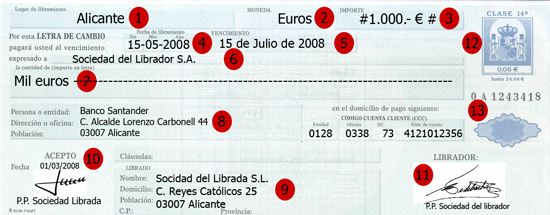
\includegraphics[width=\textwidth]{img/letra.jpg}
\caption{Ejemplo de letra de cambio obtenido de \href{http://www.abanfin.com/?tit=letra-de-cambio-caracteristicas&name=Manuales&fid=eh0bcao}{abanfin.com}.}
\label{fig:Letra}
\begin{enumerate}
  \itemsep-0em
\item Lugar de emisión.
\item Denominación de la moneda en la que se ha emitido.
\item Cuantía de la Letra.
\item Fecha de libramiento, esto es, el momento en que se ha emitido la letra de cambio.
\item Fecha de vencimiento, fecha en la que el librado, quién tiene que pagar ha de hacer efectivo el pago.
\item Librador, datos del emisor de la letra de cambio.
\item Cuantía de la letra de cambio expresada en cifra.
\item Domicilio de pago, si bien no es un requisito indispensable cuando se especifica se dice que la letra de cambio se encuentra domiciliada, suele corresponderse con la dirección de la entidad bancaria donde habrá de hacerse efectivo el pago.
\item Datos del librado, identificación y dirección de la persona, física o jurídica, que ha de realizar el pago.
\item Aceptación por parte del librado del pago, en ocasiones la letra se presenta al librado para que con su firma acepte de el visto bueno al pago.
\item Firma autógrafa del librador, esto es, del emisor de la letra de cambio.
\item Tasa de timbres - Actos Jurídicos Documentados- que se tendrán que liquidar para poner en circulación la letra. En este sentido cabe destacar que la cuantía de dicha tasa depende de la cuantía del documento.
\item Identificación del documento utilizado para su cumplimentación.
\end{enumerate}
\end{figure}




\paragraph{Endosos: }
El pago de la letra de cambio se puede realizar al librador o a un tercero llamado beneficiario, \substudy{tomador o tenedor}, a quien el librador ha transmitido o endosado la letra de cambio.
Aquel que endosa una deuda es un \textbf{endosante} y aquel a quien es endosada es un \textbf{endosatario}\footnote{Que no son insultos ninguna de las 2 palabras.}. Más formalmente, \substudy{el endoso consiste en la transmisión a un tercero de los derechos de cobro derivados de la letra de cambio}


\paragraph{Aceptación: }Tal y como dice el refranero español, 2 no se endeudan si uno no quiere. ¿Qué ocurre si el librador (cobrador,tenedor) ordena a una persona que en realidad no le debe dinero? Obviamente esto no puede ocurrir y el librado (deudor) tiene que aceptar la letra para que esta sea válida.
Sin la aceptación de la letra, no está obligado a pagar. ¿Y si no quiero aceptarla? Entonces el beneficiario (tenedor) (que podría ser otra persona distinta al librador si ha letra ha sido endosada) cargará con el peso de la ley sobre el librado. Los artículos 49 a 60 de LCCH regulan este tipo de acciones posibles a llevar a cabo.
%% TODO: Esos ... habría que rellenarlos.


La \study{aceptación} de una letra puede ser \substudy{\textbf{parcial}} o \substudy{\textbf{total}}.
Debe realizarse por \substudy{la firma de la letra} y \study{\textbf{no puede estar sujeta a ninguna condición}}.

Mientras que la \study{aceptación} puede ser \substudy{parcial}, un endoso no. Al \study{endosar} una letra, tiene que endosarse \substudy{completamente}.

\paragraph{Cláusulas en la letra: } Las letras de cambio además pueden tener cláusulas. Por ejemplo, \textit{Cuando el librador} (cobrador) \textit{haya escrito en la letra de cambio las palabras \study{«no a la orden»}, o una expresión equivalente, \substudy{el título no será transmisible}, \substudy{sino} en la forma y con los efectos de una \substudy{cesión ordinaria}.}
\footnote{Una cesión ordinaria es una trasmisión de un derecho. Al ser una cesión ordinaria y no un endoso, se le aplicará la ley que hable de cesiones y no de endosos.} (\href{https://www.boe.es/buscar/act.php?id=BOE-A-1985-14880&p=20150703&tn=1#acatorce}{Art 14, LCCH})

Otro ejemplo (\href{https://www.boe.es/buscar/act.php?id=BOE-A-1985-14880&p=20150703&tn=1#acatorce}{Art 18, LCCH}) \textit{El endosante, salvo cláusula en contrario, garantiza la aceptación y el pago frente a los tenedores posteriores. \substudy{El endosante puede prohibir un nuevo endoso}. En este caso, \study{no responderá} frente a las personas a quienes \study{ulteriormente} se endosare la letra.}

\paragraph{Intereses: }

No todas las letras de cambio son iguales. Algunas pueden incorporar intereses, tal y como regula el \href{https://www.boe.es/buscar/act.php?id=BOE-A-1985-14880&p=20150703&tn=1#asexto}{art. 6 de LCCH}, que al parecer es habitual.

\paragraph{Sobre el pago de la letra: }

Todos los endosos deberán llevar la firma tanto del endosante como del endosatario, dando lugar a una traza de los endosos. De esta manera, el último tenedor (cobrador) es quien puede ejercer el derecho de cobro.


El pago de la letra se efectuará en la fecha de vencimiento (que tiene que estar incluida en la letra) y será un pago total.


No obstante, se contempla la posibilidad de que el tomador (o beneficiario) de una letra (quién tiene que recibirla) pueda cobrarla antes de que venza.
Esta operación, denominada \textbf{\study{descuento}}, es una operación de crédito mediante la cual una entidad financiera (\substudy{no pueden ser personas físicas}) anticipa el importe no vencido (menos los intereses) de la letra de cambio a cambio de la cesión o endoso de la misma (habitualmente con cobro de comisión).
De esta manera, el tomador (o beneficiario) puede obtener liquidez inmediata y no esperar al vencimiento de la letra de cambio para que el dinero se haga efectivo.
Así, las \textbf{\study{consecuencias}} de un descuento son: al librado ni le va ni le viene. Paga lo mismo que tenía que pagar en la fecha de vencimiento. El beneficiario recibe liquidez por un importe menor al de la letra. La entidad financiera externa gana dinero.





\subsubsection{Letras del tesoro}
Las Letras del Tesoro son activos a corto plazo emitidos por el Tesoro Público para financiar el déficit público. Son una de las principales fuentes de financiación de los gobiernos.
Se emiten a plazos muy cortos: 3, 6, 9 y 12 meses.

Las Letras del Tesoro \study{se emiten "al descuento"}, lo que significa que se descuenta al inversor el importe de los intereses en el momento de la compra.

Por ejemplo, compramos una Letra a un año con un valor nominal de 1.000 \texteuro, pero pagando un precio inferior; por ejemplo, 970 \texteuro.
Cuando vence la Letra podremos reembolsarla por su valor nominal (1.000 \texteuro), por lo que habremos obtenido una ganancia de 30 \texteuro.
Pero, ¿por qué hemos podido comprar la letra por menos valor? Porque las Letras del Tesoro se emiten en subastas. De esta manera, quien invierte gana dinero y el Estado gana liquidez. \substudy{Las Letras del Tesoro se consideran la inversión financiera de mayor seguridad y liquidez del mercado monetario.}


\subsubsection{Factoring}

Es una operación financiera que consiste en la cesión a un factor (empresa de "factoring") de créditos comerciales\footnote{Las letras de cambio son créditos comerciales.} por parte de una empresa, a cambio de un importe convenido.
La sociedad especializada (denominada factor) asume el riesgo de insolvencia del crédito y se encarga de su cobro a cambio de una comisión de "factorage" sobre el importe de la factura.

Si te parece que es exactamente lo mismo el factoring que un descuento, vas por buen camino querido lector. Vamos a ver los matices que los diferencian para poder utilizar estas palabras pensando que sabemos de lo que hablamos.

Un descuento es una operación que se basa en un efecto comercial (la letra o similar), mientras que el \study{factoring} se basa en la \substudy{prestación de servicios}. Yo como "factor" ofrezco un servicio de gestión y cobro de pagos y deudas, aunque el modo de proceder sea similar. En ambos casos, tanto el banco como el factor, pagan el importe de la deuda por adelantado que se cobrará en un futuro. La consecuencia de que \substudy{el "factor"} ofrezca un servicio es que \substudy{puede hacer un poco lo que le de la gana}. Puede pagar a plazos el importe, puede ocuparse de la gestión en caso de impago o no, etc

Por ejemplo, sea una empresa $A$ que ofrece un servicio a muchos clientes distintos. La empresa $A$ puede contratar a una empresa de factoring ($B$) a quien cede todas las deudas a cambio de liquidez inmediata y es la empresa $B$ quien gestiona los cobros y quien asume los impagos. De esta manera $A$, aunque gane menos dinero,  obtiene mayor liquidez y menor gasto en administración de cobros.


En la tabla \ref{tab:FactoringVsDescuento} encontramos varias diferencias de manera más esquemática y clara.

\begin{table}[hbtp]
\centering
\begin{tabular}{r||l|l}
&\textbf{Factoring} &\textbf{Descuento} \\
\toprule
Documento & Factura & Letra de cambio\\
Pago anticipado & Flexible & A tocateja\\
Cobertura de impago & Es posible\footnote{En caso de ser factoring sin recurso, la cobertura de pago está incluida. Si el factoring es con recurso, entonces no. (Con recurso implica que la empresa de factor puede quejarse a ti, que le has contratado y recurrir esa deuda).} & No\\
Otros servicios & Es posible\footnote{Depende del contrato de factoring que contrates y con quien lo contrates.} & No
\end{tabular}
\caption{\study{Diferencias entre Factoring y descuento bancario}}
\label{tab:FactoringVsDescuento}
\end{table}

\obs En caso de que una empresa de factoring esté dispuesta a asumir los impagos, ésta querrá asegurarse que los deudores van a pagar las deudas.
En ese caso, la empresa de factoring contratada limitará los negocios de quien le haya contratado para que sólo haga negocios con empresa confiables.

\section{Evaluación de proyectos de inversión}

A la hora de evaluar si llevar a cabo un proyecto o no, necesitaremos ciertos indicadores que nos permitan saber si ese proyecto puede ser rentable o no. No vale simplemente con sumar los ingresos previstos y restarle los gastos: como vimos en la sección anterior, el valor del dinero cambia con el tiempo, así que nos interesará saber además en cuánto tiempo vamos a recuperar la inversión.

El primer indicador y el más simple es el \concept{Plazo\IS de recuperación} (PR), que no es más que el tiempo que ha de pasar hasta que recuperemos todo lo que hemos invertido. Si consideramos que es un plazo demasiado largo, rechazamos el proyecto.

Sin embargo, necesitamos algo más si queremos hacer una evaluación completa. El plazo de recuperación no nos distinguiría entre dos proyectos que cuestan lo mismo y dan los mismos beneficios anuales, pero con uno de ellos dando beneficios durante más tiempo.

Aquí entran en juego dos indicadores duales, el \concept{Valor\IS Actual Neto} (VAN) y la \concept{Tasa\IS Interna de Rendimiento} (TIR), ambos relacionados por la siguiente ecuación:
\[ \mathrm{VAN} = \sum_{k=0}^n \frac{C_k}{(1+\mathrm{r})^k}\], donde $C_k$ es el flujo de dinero en el período $k$ (normalmente, en el período 0 sólo tenemos gastos porque es la inversión inicial) y $r$ es la tasa de actualización. El TIR es la tasa de actualización que hace que el VAN sea cero.

El VAN es el valor actualizado de todos los flujos de caja. Obviamente, si el VAN es negativo estamos ante un proyecto que no es viable. El problema es que requiere fijar la tasa de actualización. Habitualmente, se usa como mínimo el coste del capital, es decir, el porcentaje de ``intereses'' anuales que ha de pagar una compañía para financiarse\footnote{Esto incluye intereses de préstamos, pero también el retorno que esperan los accionistas, por ejemplo.}. Es decir, buscamos ganar más dinero del que sacamos obteniendo financiación por las vías habituales.

El TIR es, como decíamos, un valor dual al del VAN: es la tasa de actualización que hace que el VAN sea cero. Si el TIR es mayor que nuestro coste del capital, consideraremos que el proyecto es rentable. El problema es que es ligeramente más complejo de calcular (necesitaremos resolver la ecuación numéricamente en la mayoría de los casos) y según las condiciones de la ecuación (por ejemplo, con algunos flujos de caja negativos en medio del proyecto) puede dar múltiples soluciones.

Otro problema de estos dos indicadores es que asumen que los flujos de caja se reinvierten hasta el último período con el mismo tipo de interés que la tasa de actualización. Si podemos invertir los beneficios a un tipo de interés mayor que la tasa de actualización, nos beneficiaremos de tener los flujos de caja positivos cuanto antes posible, para invertirlos antes y sacar más dinero. Sin embargo, esto no lo tiene en cuenta el VAN y podríamos obtener resultados anómalos.

Aparte de estos, tenemos otros indicadores más avanzados para proyectos de inversión. El primero es el \concept{{Í}ndice\IS de rentabilidad}, que lo que hace es medir el ratio del VAN entre la inversión inicial. Este índice nos dice cuánto ganamos por cada unidad invertida, permitiendo así la comparación más sencilla entre inversiones con costes iniciales y duraciones diferentes.

% Esta mierda viene explicada fatal en Internet y no sé cómo se traduce al inglés así que paso de mirarlo más. No tiene ningún sentido

También resulta de cierto interés la \concept{Tasa\IS de Fisher} para comparar dos proyectos de inversión. Es la tasa de actualización para la cual ambos tienen el mismo VAN. Si la tasa de Fisher es mayor que la tasa de actualización que consideramos para el VAN, tendremos que el TIR y el VAN nos dan cada uno un proyecto ``mejor''. Habitualmente, es el VAN al que deberíamos hacer caso, aunque la tasa de Fisher nos dará una idea de cómo de diferentes son los proyectos.

\section{Mercado y márketing}

Esta sección no ha tenido especial peso en el desarrollo de este curso. Nos hemos limitado a dar algunas pinceladas a algunos conceptos relacionados con el Marketing.

\subsection{Tipos de mercado}

Existen 4 tipos de mercados principalmente:
\begin{itemize}
\item \textbf{Competencia perfecta}. Existen numerosas empresas que pelean en igualdad de condiciones y los precios fluctúan en función de la oferta y la demanda. Todas las empresas compiten por ofrecer lo mejor a sus clientes. La demanda es atómica, hay sustitutivos perfectos (no hay productos insustituibles) y no hay barreras, falta de información ni costes de transacción.

\item \textbf{Competencia monopolística}
Es un tipo de competencia en la que existe una cantidad significativa de productores actuando en el mercado sin que exista un control dominante por parte de ninguno de estos en particular. Ésta es muy frecuente dentro de los mercados de productos que se encuentran normalmente en los supermercados, donde existen productos de diferentes marcas, pero con características particulares y dentro de cada grupo de producto, las características los hacen diferentes unos de otros, pero lo suficientemente parecidos para competir con otros productores y entre sí.
\item \textbf{Oligopolio homogéneo y diferenciado}
Existen muy pocas empresas pero sus productos son muy parecidos entre si.
\item \textbf{Monopolio}
Existe una única empresa que controla todo el mercado, con lo que puede modificar los precios a su antojo sabiendo que los clientes no tienen otra opción.
\end{itemize}

\subsection{Segmentación y público objetivo}

A la hora de buscar nuestros clientes, es importante segmentarlos y ver concretamente a qué sector queremos dirigirnos. Por ejemplo, quizás querramos ir sólo a por los clientes de una zona geográfica concreta, a los de un cierto nivel de renta, con un estilo de vida específico... Una vez entendido nuestro público objetivo, sabremos cómo dirigirnos a él, cuáles son sus influencias\footnote{Por ejemplo, si queremos gente que le guste la moda, estarán influenciado por \textit{bloggers de moda}. Buscaremos entonces que la publicidad nos la hagan \textit{bloggers de moda} para así tener más influencia y montar un markéting más efectivo.} y cómo modelar el producto para que cumpla las necesidades del cliente (aunque en realidad nos basta con que el cliente quede convencido de ello).

\subsection{Cuatro P's: Producto, Precio, Promoción y Distribución (Placement)}

Las cuatro P's del Márketing son una forma de ver cómo vender un producto modificando alguna de las cuatro variables.

La primera es el \textbf{producto}: lo que vendemos al cliente. Tenemos que ajustarlo para que sirva a los clientes, y tener en cuenta también su ciclo de vida. Además, es interesante conocer la curva de adopción de la tecnología: al principio tenemos unos pocos innovadores y \textit{early adopters}, muy informados y que buscan tecnología y rendimiento. Después se da el salto a las mayorías: primero la precoz, luego los conservadores y por último llegando a los escépticos. Estos usuarios buscan más bien comodidad y buena experiencia de usuario, y no se preocupan tanto por estar a la última.

La segunda variable es el \textbf{precio}, que podremos establecer basándonos en los costes, en el comprador (ponemos el precio que nuestro comprador objetivo pueda comprar) o en la competencia, para evitar perder cuota de mercado.

Aquí entra en juego el concepto de la \concept{Elasticidad\IS de precio}, que nos dice cómo responde la demanda a cambios en el precio. La ecuación es simplemente el cociente entre el cambio en demanda y el cambio en precio, ambos expresados como porcentaje. Una elasticidad entre 0 y 1 nos da una demanda rígida o no elástica: la subida en precio no se refleja en una bajada drástica en demanda. En este caso, subir el precio implica una subida en beneficios. Se suele dar cuando el producto es necesario, cuando no hay sustitutos posibles o cuando hay lealtad a una marca, entre otras razones. Un ejemplo de este caso sería la electricidad: la demanda variará poco con la variación de precio.

Por el contrario, una demanda elástica (mayor que 1) se da en mercados con mayor competencia, e indica que cuanto más se suba el precio menos demanda se tendrá y perderemos beneficios

La tercera variable, la \textbf{distribución}, hace referencia a la facilidad de los clientes para acceder y comprar nuestro producto. Por ejemplo, si tenemos un producto muy bueno a muy buen precio pero que sólo vendemos en nuestra tienda física de Villaplatos de Arriba, no vamos a vender demasiado. Por el contrario, si tenemos tiendas \textit{online} u otros modos de distribución efectiva, conseguiremos más clientes aunque no tengamos el mejor producto.

Por último, la \textbf{promoción} es importante para que los clientes sepan que nuestro producto exista. Tenemos vendedores, relaciones públicas, publicidad, patrocinios, promociones, etc. En Internet es importante saber cómo posicionarse. Por un lado, tenemos el SEO (\textit{Search Engine Optimization}) que busca colocarse en lo más alto en los resultados de búsqueda para ciertas palabras clave. Una gran parte del tráfico de una web viene de los motores de búsqueda, así que este es un aspecto importante.

También es posible comprar anuncios para aparecer en los resultados patrocinados y también para aparecer en otras páginas web que coloquen anuncios. En este sentido es importante la selección de palabras claves, ya que nos permitirán obtener la mejor tasa de conversión (queremos que los usuarios que hagan clic sean sólo los interesados y que además nos compren cosas) sin ir a palabras demasiado genéricas con un coste por anuncio más elevado.

\subsection{Caso de estudio: Jamming}

De cara al desarrollo y comercialización de un producto, atendimos a la charla dada por unos compañeros que desarrollaron una aplicación llamada \href{buscarurl}{Jamming}.

Uno de los conceptos más importante que pudimos sacar en limpio de esta charla (y que no hayamos mencionado ya a lo largo de estos apuntes) es el concepto de \concept{Producto mínimo viable}. La idea es sencilla: No podemos esperar hasta que el producto está absolutamente completado para sacarlo a la venta pues pueden adelantarse y robarnos la idea y, en caso de salir mal el negocio, habremos invertido demasiado tiempo.

El objetivo de este producto mínimo viable es poder presentar algo a los clientes de forma que podamos empezar a obtener feed back lo antes posible, garanticemos nuestro hueco en el mercado, y podamos centrar nuestros esfuerzos en los aspectos que realmente están funcionando.

\printindex
\end{document}
